\documentclass[1p]{elsarticle_modified}
%\bibliographystyle{elsarticle-num}

%\usepackage[colorlinks]{hyperref}
%\usepackage{abbrmath_seonhwa} %\Abb, \Ascr, \Acal ,\Abf, \Afrak
\usepackage{amsfonts}
\usepackage{amssymb}
\usepackage{amsmath}
\usepackage{amsthm}
\usepackage{scalefnt}
\usepackage{amsbsy}
\usepackage{kotex}
\usepackage{caption}
\usepackage{subfig}
\usepackage{color}
\usepackage{graphicx}
\usepackage{xcolor} %% white, black, red, green, blue, cyan, magenta, yellow
\usepackage{float}
\usepackage{setspace}
\usepackage{hyperref}

\usepackage{tikz}
\usetikzlibrary{arrows}

\usepackage{multirow}
\usepackage{array} % fixed length table
\usepackage{hhline}

%%%%%%%%%%%%%%%%%%%%%
\makeatletter
\renewcommand*\env@matrix[1][\arraystretch]{%
	\edef\arraystretch{#1}%
	\hskip -\arraycolsep
	\let\@ifnextchar\new@ifnextchar
	\array{*\c@MaxMatrixCols c}}
\makeatother %https://tex.stackexchange.com/questions/14071/how-can-i-increase-the-line-spacing-in-a-matrix
%%%%%%%%%%%%%%%

\usepackage[normalem]{ulem}

\newcommand{\msout}[1]{\ifmmode\text{\sout{\ensuremath{#1}}}\else\sout{#1}\fi}
%SOURCE: \msout is \stkout macro in https://tex.stackexchange.com/questions/20609/strikeout-in-math-mode

\newcommand{\cancel}[1]{
	\ifmmode
	{\color{red}\msout{#1}}
	\else
	{\color{red}\sout{#1}}
	\fi
}

\newcommand{\add}[1]{
	{\color{blue}\uwave{#1}}
}

\newcommand{\replace}[2]{
	\ifmmode
	{\color{red}\msout{#1}}{\color{blue}\uwave{#2}}
	\else
	{\color{red}\sout{#1}}{\color{blue}\uwave{#2}}
	\fi
}

\newcommand{\Sol}{\mathcal{S}} %segment
\newcommand{\D}{D} %diagram
\newcommand{\A}{\mathcal{A}} %arc


%%%%%%%%%%%%%%%%%%%%%%%%%%%%%5 test

\def\sl{\operatorname{\textup{SL}}(2,\Cbb)}
\def\psl{\operatorname{\textup{PSL}}(2,\Cbb)}
\def\quan{\mkern 1mu \triangleright \mkern 1mu}

\theoremstyle{definition}
\newtheorem{thm}{Theorem}[section]
\newtheorem{prop}[thm]{Proposition}
\newtheorem{lem}[thm]{Lemma}
\newtheorem{ques}[thm]{Question}
\newtheorem{cor}[thm]{Corollary}
\newtheorem{defn}[thm]{Definition}
\newtheorem{exam}[thm]{Example}
\newtheorem{rmk}[thm]{Remark}
\newtheorem{alg}[thm]{Algorithm}

\newcommand{\I}{\sqrt{-1}}
\begin{document}

%\begin{frontmatter}
%
%\title{Boundary parabolic representations of knots up to 8 crossings}
%
%%% Group authors per affiliation:
%\author{Yunhi Cho} 
%\address{Department of Mathematics, University of Seoul, Seoul, Korea}
%\ead{yhcho@uos.ac.kr}
%
%
%\author{Seonhwa Kim} %\fnref{s_kim}}
%\address{Center for Geometry and Physics, Institute for Basic Science, Pohang, 37673, Korea}
%\ead{ryeona17@ibs.re.kr}
%
%\author{Hyuk Kim}
%\address{Department of Mathematical Sciences, Seoul National University, Seoul 08826, Korea}
%\ead{hyukkim@snu.ac.kr}
%
%\author{Seokbeom Yoon}
%\address{Department of Mathematical Sciences, Seoul National University, Seoul, 08826,  Korea}
%\ead{sbyoon15@snu.ac.kr}
%
%\begin{abstract}
%We find all boundary parabolic representation of knots up to 8 crossings.
%
%\end{abstract}
%\begin{keyword}
%    \MSC[2010] 57M25 
%\end{keyword}
%
%\end{frontmatter}

%\linenumbers
%\tableofcontents
%
\newcommand\colored[1]{\textcolor{white}{\rule[-0.35ex]{0.8em}{1.4ex}}\kern-0.8em\color{red} #1}%
%\newcommand\colored[1]{\textcolor{white}{ #1}\kern-2.17ex	\textcolor{white}{ #1}\kern-1.81ex	\textcolor{white}{ #1}\kern-2.15ex\color{red}#1	}

{\Large $\underline{12a_{0460}~(K12a_{0460})}$}

\setlength{\tabcolsep}{10pt}
\renewcommand{\arraystretch}{1.6}
\vspace{1cm}\begin{tabular}{m{100pt}>{\centering\arraybackslash}m{274pt}}
\multirow{5}{120pt}{
	\centering
	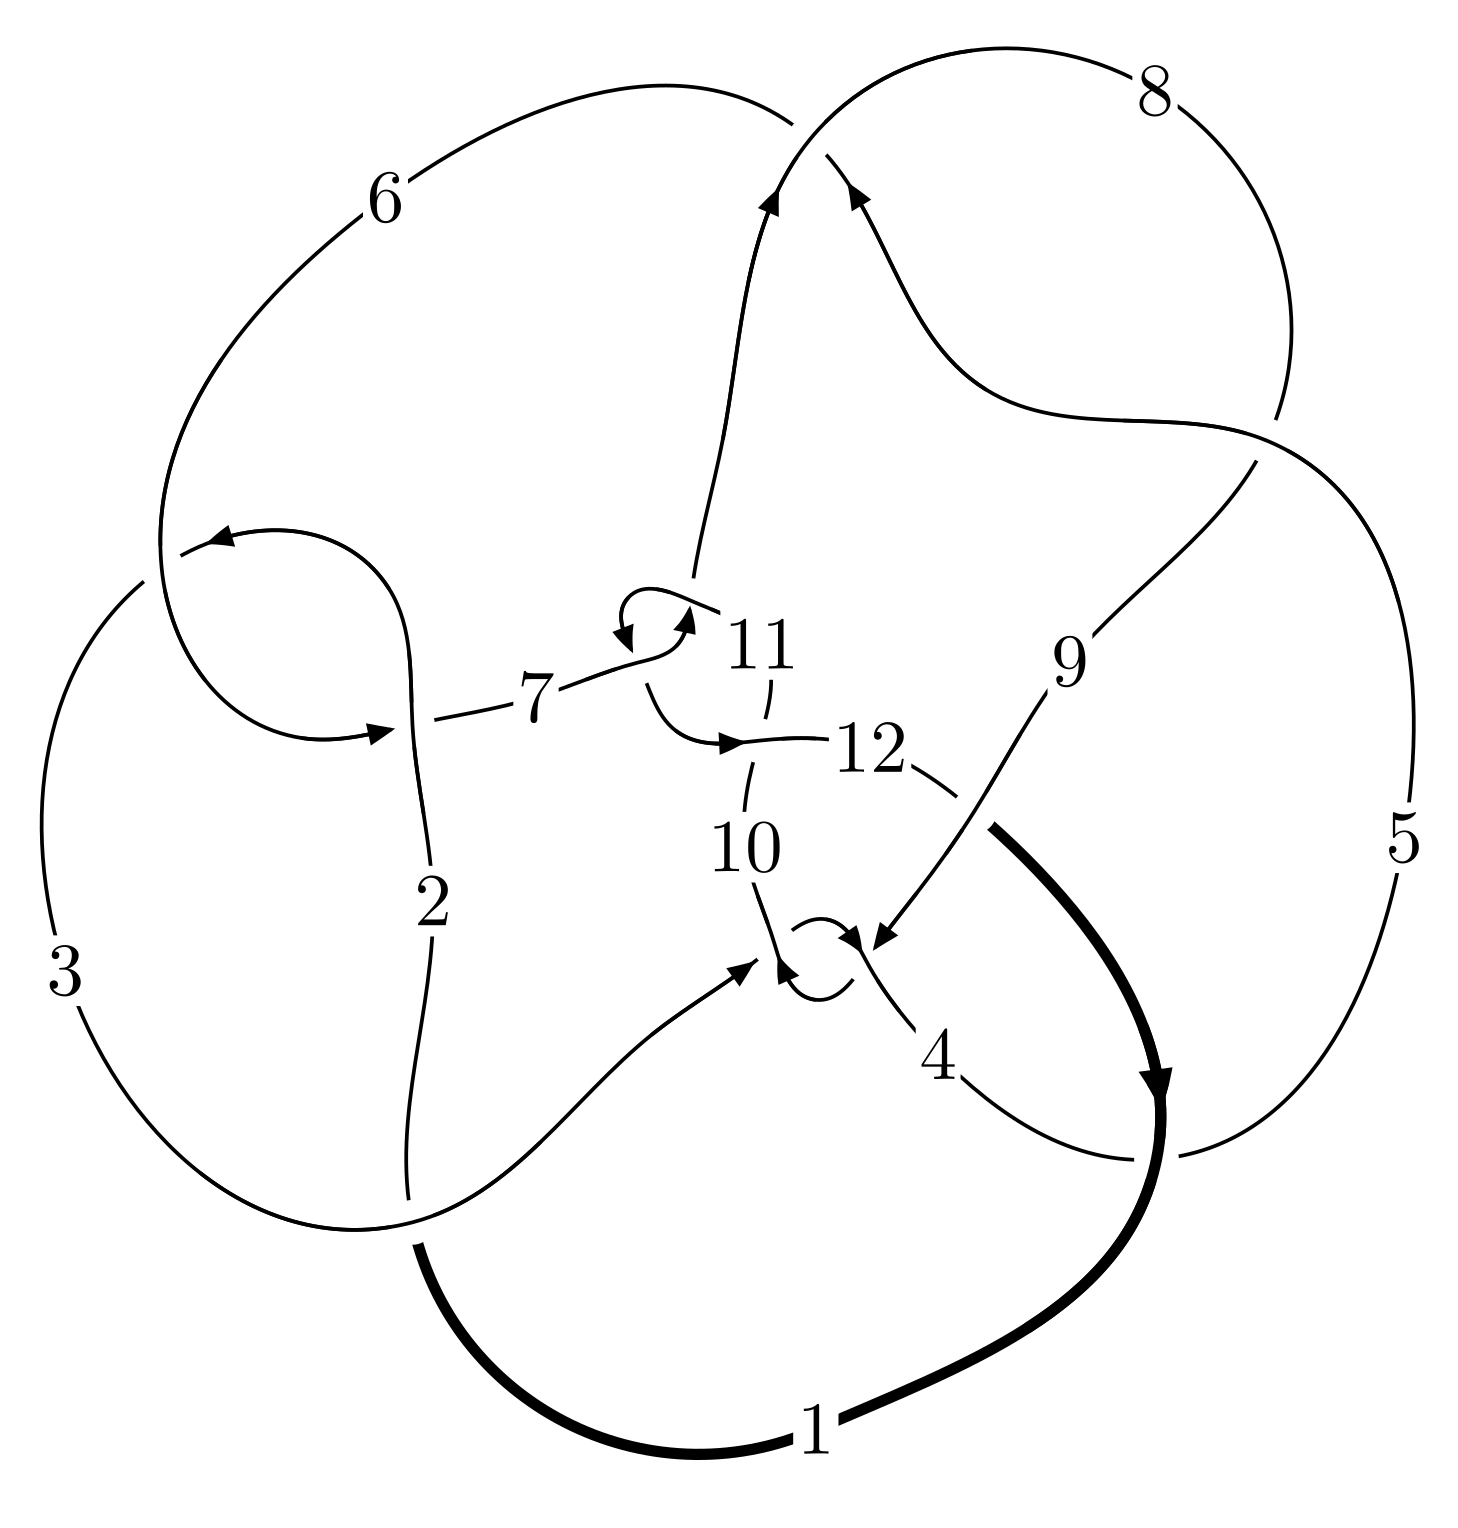
\includegraphics[width=112pt]{../../../GIT/diagram.site/Diagrams/png/1261_12a_0460.png}\\
\ \ \ A knot diagram\footnotemark}&
\allowdisplaybreaks
\textbf{Linearized knot diagam} \\
\cline{2-2}
 &
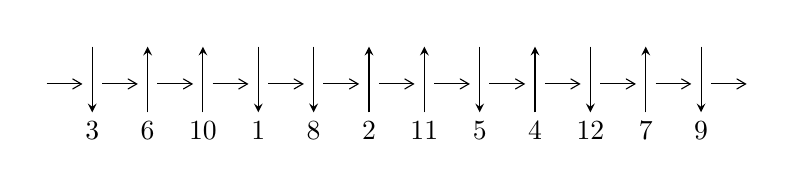
\begin{tikzpicture}[x=20pt, y=17pt]
	% nodes
	\node (C0) at (0, 0) {};
	\node (C1) at (1, 0) {};
	\node (C1U) at (1, +1) {};
	\node (C1D) at (1, -1) {3};

	\node (C2) at (2, 0) {};
	\node (C2U) at (2, +1) {};
	\node (C2D) at (2, -1) {6};

	\node (C3) at (3, 0) {};
	\node (C3U) at (3, +1) {};
	\node (C3D) at (3, -1) {10};

	\node (C4) at (4, 0) {};
	\node (C4U) at (4, +1) {};
	\node (C4D) at (4, -1) {1};

	\node (C5) at (5, 0) {};
	\node (C5U) at (5, +1) {};
	\node (C5D) at (5, -1) {8};

	\node (C6) at (6, 0) {};
	\node (C6U) at (6, +1) {};
	\node (C6D) at (6, -1) {2};

	\node (C7) at (7, 0) {};
	\node (C7U) at (7, +1) {};
	\node (C7D) at (7, -1) {11};

	\node (C8) at (8, 0) {};
	\node (C8U) at (8, +1) {};
	\node (C8D) at (8, -1) {5};

	\node (C9) at (9, 0) {};
	\node (C9U) at (9, +1) {};
	\node (C9D) at (9, -1) {4};

	\node (C10) at (10, 0) {};
	\node (C10U) at (10, +1) {};
	\node (C10D) at (10, -1) {12};

	\node (C11) at (11, 0) {};
	\node (C11U) at (11, +1) {};
	\node (C11D) at (11, -1) {7};

	\node (C12) at (12, 0) {};
	\node (C12U) at (12, +1) {};
	\node (C12D) at (12, -1) {9};
	\node (C13) at (13, 0) {};

	% arrows
	\draw[->,>={angle 60}]
	(C0) edge (C1) (C1) edge (C2) (C2) edge (C3) (C3) edge (C4) (C4) edge (C5) (C5) edge (C6) (C6) edge (C7) (C7) edge (C8) (C8) edge (C9) (C9) edge (C10) (C10) edge (C11) (C11) edge (C12) (C12) edge (C13) ;	\draw[->,>=stealth]
	(C1U) edge (C1D) (C2D) edge (C2U) (C3D) edge (C3U) (C4U) edge (C4D) (C5U) edge (C5D) (C6D) edge (C6U) (C7D) edge (C7U) (C8U) edge (C8D) (C9D) edge (C9U) (C10U) edge (C10D) (C11D) edge (C11U) (C12U) edge (C12D) ;
	\end{tikzpicture} \\
\hhline{~~} \\& 
\textbf{Solving Sequence} \\ \cline{2-2} 
 &
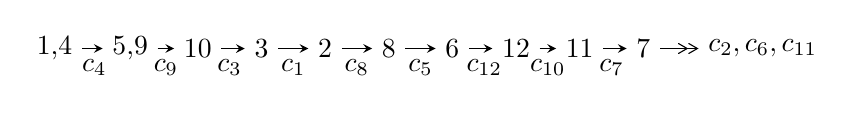
\begin{tikzpicture}[x=23pt, y=7pt]
	% node
	\node (A0) at (-1/8, 0) {1,4};
	\node (A1) at (17/16, 0) {5,9};
	\node (A2) at (17/8, 0) {10};
	\node (A3) at (25/8, 0) {3};
	\node (A4) at (33/8, 0) {2};
	\node (A5) at (41/8, 0) {8};
	\node (A6) at (49/8, 0) {6};
	\node (A7) at (57/8, 0) {12};
	\node (A8) at (65/8, 0) {11};
	\node (A9) at (73/8, 0) {7};
	\node (C1) at (1/2, -1) {$c_{4}$};
	\node (C2) at (13/8, -1) {$c_{9}$};
	\node (C3) at (21/8, -1) {$c_{3}$};
	\node (C4) at (29/8, -1) {$c_{1}$};
	\node (C5) at (37/8, -1) {$c_{8}$};
	\node (C6) at (45/8, -1) {$c_{5}$};
	\node (C7) at (53/8, -1) {$c_{12}$};
	\node (C8) at (61/8, -1) {$c_{10}$};
	\node (C9) at (69/8, -1) {$c_{7}$};
	\node (A10) at (11, 0) {$c_{2},c_{6},c_{11}$};

	% edge
	\draw[->,>=stealth]	
	(A0) edge (A1) (A1) edge (A2) (A2) edge (A3) (A3) edge (A4) (A4) edge (A5) (A5) edge (A6) (A6) edge (A7) (A7) edge (A8) (A8) edge (A9) ;
	\draw[->>,>={angle 60}]	
	(A9) edge (A10);
\end{tikzpicture} \\ 

\end{tabular} \\

\footnotetext{
The image of knot diagram is generated by the software ``\textbf{Draw programme}" developed by Andrew Bartholomew(\url{http://www.layer8.co.uk/maths/draw/index.htm\#Running-draw}), where we modified some parts for our purpose(\url{https://github.com/CATsTAILs/LinksPainter}).
}\phantom \\ \newline 
\centering \textbf{Ideals for irreducible components\footnotemark of $X_{\text{par}}$} 
 
\begin{align*}
I^u_{1}&=\langle 
2.48339\times10^{23} u^{25}-2.92787\times10^{23} u^{24}+\cdots+5.04980\times10^{23} b+1.13922\times10^{24},\;a-1,\;u^{26}- u^{25}+\cdots+u+1\rangle \\
I^u_{2}&=\langle 
2.42800\times10^{731} u^{107}-2.38703\times10^{732} u^{106}+\cdots+1.67435\times10^{731} b-2.81845\times10^{733},\\
\phantom{I^u_{2}}&\phantom{= \langle  }7.28015\times10^{733} u^{107}-1.32007\times10^{734} u^{106}+\cdots+1.67435\times10^{731} a+3.97573\times10^{733},\\
\phantom{I^u_{2}}&\phantom{= \langle  }u^{108}-2 u^{107}+\cdots-20 u+1\rangle \\
I^u_{3}&=\langle 
-10 u^{11}-2 u^{10}-3 u^9-4 u^8-75 u^7-20 u^6-18 u^5-14 u^4-138 u^3-46 u^2+9 b-22 u+10,\;a+1,\\
\phantom{I^u_{3}}&\phantom{= \langle  }u^{12}+u^{11}+u^{10}+u^9+8 u^8+8 u^7+7 u^6+5 u^5+16 u^4+16 u^3+12 u^2+4 u+1\rangle \\
I^u_{4}&=\langle 
-2970 u^{11}-16830 u^{10}+\cdots+3431 b-12700,\;2891 u^{11}+14095 u^{10}+\cdots+3431 a+4241,\\
\phantom{I^u_{4}}&\phantom{= \langle  }u^{12}+5 u^{11}+11 u^{10}+15 u^9+11 u^8+7 u^7+11 u^6+10 u^5+22 u^4+17 u^3+12 u^2+4 u+1\rangle \\
\\
\end{align*}
\raggedright * 4 irreducible components of $\dim_{\mathbb{C}}=0$, with total 158 representations.\\
\footnotetext{All coefficients of polynomials are rational numbers. But the coefficients are sometimes approximated in decimal forms when there is not enough margin.}
\newpage
\renewcommand{\arraystretch}{1}
\centering \section*{I. $I^u_{1}= \langle 2.48\times10^{23} u^{25}-2.93\times10^{23} u^{24}+\cdots+5.05\times10^{23} b+1.14\times10^{24},\;a-1,\;u^{26}- u^{25}+\cdots+u+1 \rangle$}
\flushleft \textbf{(i) Arc colorings}\\
\begin{tabular}{m{7pt} m{180pt} m{7pt} m{180pt} }
\flushright $a_{1}=$&$\begin{pmatrix}0\\u\end{pmatrix}$ \\
\flushright $a_{4}=$&$\begin{pmatrix}1\\0\end{pmatrix}$ \\
\flushright $a_{5}=$&$\begin{pmatrix}1\\u^2\end{pmatrix}$ \\
\flushright $a_{9}=$&$\begin{pmatrix}1\\-0.491779 u^{25}+0.579798 u^{24}+\cdots-0.505057 u-2.25597\end{pmatrix}$ \\
\flushright $a_{10}=$&$\begin{pmatrix}-0.491779 u^{25}+0.579798 u^{24}+\cdots-0.505057 u-1.25597\\-0.491779 u^{25}+0.579798 u^{24}+\cdots-0.505057 u-2.25597\end{pmatrix}$ \\
\flushright $a_{3}=$&$\begin{pmatrix}1.04793 u^{25}-1.22784 u^{24}+\cdots+1.46589 u+1.80094\\1.53971 u^{25}-1.80763 u^{24}+\cdots+1.97095 u+3.05691\end{pmatrix}$ \\
\flushright $a_{2}=$&$\begin{pmatrix}-0.145439 u^{25}-0.0814371 u^{24}+\cdots+9.19172 u+0.529548\\-0.0826126 u^{25}-0.323908 u^{24}+\cdots+13.6227 u+1.32755\end{pmatrix}$ \\
\flushright $a_{8}=$&$\begin{pmatrix}-0.491779 u^{25}+0.579798 u^{24}+\cdots-0.505057 u-1.25597\\-0.544904 u^{25}+0.618776 u^{24}+\cdots-0.101297 u-2.34399\end{pmatrix}$ \\
\flushright $a_{6}=$&$\begin{pmatrix}1.15418 u^{25}-1.30579 u^{24}+\cdots+0.658374 u+1.97698\\1.81723 u^{25}-2.07044 u^{24}+\cdots+0.160858 u+3.38456\end{pmatrix}$ \\
\flushright $a_{12}=$&$\begin{pmatrix}u\\0.0880194 u^{25}-0.141144 u^{24}+\cdots-0.764194 u+0.491779\end{pmatrix}$ \\
\flushright $a_{11}=$&$\begin{pmatrix}-0.326147 u^{25}+0.397989 u^{24}+\cdots-1.37309 u-1.07607\\-0.671424 u^{25}+0.829108 u^{24}+\cdots+0.230116 u-2.31880\end{pmatrix}$ \\
\flushright $a_{7}=$&$\begin{pmatrix}-0.0777366 u^{25}+0.193064 u^{24}+\cdots-1.97629 u-0.609278\\-0.108030 u^{25}+0.293691 u^{24}+\cdots-3.45433 u-1.07896\end{pmatrix}$\\&\end{tabular}
\flushleft \textbf{(ii) Obstruction class $= -1$}\\~\\
\flushleft \textbf{(iii) Cusp Shapes $= -\frac{1877165613022592980724169}{504980160038115323854327} u^{25}+\frac{3778465665043053085315905}{504980160038115323854327} u^{24}+\cdots+\frac{4750472667547566317292293}{504980160038115323854327} u-\frac{15093780059339179500460468}{504980160038115323854327}$}\\~\\
\newpage\renewcommand{\arraystretch}{1}
\flushleft \textbf{(iv) u-Polynomials at the component}\newline \\
\begin{tabular}{m{50pt}|m{274pt}}
Crossings & \hspace{64pt}u-Polynomials at each crossing \\
\hline $$\begin{aligned}c_{1},c_{10}\end{aligned}$$&$\begin{aligned}
&u^{26}+12 u^{25}+\cdots+4 u+1
\end{aligned}$\\
\hline $$\begin{aligned}c_{2},c_{6},c_{7}\\c_{11}\end{aligned}$$&$\begin{aligned}
&u^{26}+6 u^{24}+\cdots+2 u^2+1
\end{aligned}$\\
\hline $$\begin{aligned}c_{3},c_{9}\end{aligned}$$&$\begin{aligned}
&u^{26}-19 u^{25}+\cdots-480 u+64
\end{aligned}$\\
\hline $$\begin{aligned}c_{4},c_{12}\end{aligned}$$&$\begin{aligned}
&u^{26}- u^{25}+\cdots+u+1
\end{aligned}$\\
\hline $$\begin{aligned}c_{5},c_{8}\end{aligned}$$&$\begin{aligned}
&u^{26}-20 u^{25}+\cdots-3200 u+256
\end{aligned}$\\
\hline
\end{tabular}\\~\\
\newpage\renewcommand{\arraystretch}{1}
\flushleft \textbf{(v) Riley Polynomials at the component}\newline \\
\begin{tabular}{m{50pt}|m{274pt}}
Crossings & \hspace{64pt}Riley Polynomials at each crossing \\
\hline $$\begin{aligned}c_{1},c_{10}\end{aligned}$$&$\begin{aligned}
&y^{26}+12 y^{25}+\cdots+52 y+1
\end{aligned}$\\
\hline $$\begin{aligned}c_{2},c_{6},c_{7}\\c_{11}\end{aligned}$$&$\begin{aligned}
&y^{26}+12 y^{25}+\cdots+4 y+1
\end{aligned}$\\
\hline $$\begin{aligned}c_{3},c_{9}\end{aligned}$$&$\begin{aligned}
&y^{26}+7 y^{25}+\cdots+113664 y+4096
\end{aligned}$\\
\hline $$\begin{aligned}c_{4},c_{12}\end{aligned}$$&$\begin{aligned}
&y^{26}- y^{25}+\cdots-13 y+1
\end{aligned}$\\
\hline $$\begin{aligned}c_{5},c_{8}\end{aligned}$$&$\begin{aligned}
&y^{26}+8 y^{25}+\cdots+376832 y+65536
\end{aligned}$\\
\hline
\end{tabular}\\~\\
\newpage\flushleft \textbf{(vi) Complex Volumes and Cusp Shapes}
$$\begin{array}{c|c|c}  
\text{Solutions to }I^u_{1}& \I (\text{vol} + \sqrt{-1}CS) & \text{Cusp shape}\\
 \hline 
\begin{aligned}
u &= \phantom{-}0.980147 + 0.493143 I \\
a &= \phantom{-}1.00000\phantom{ +0.000000I} \\
b &= -0.097435 + 1.302150 I\end{aligned}
 & -8.66439 + 2.11653 I & -9.55328 - 2.96629 I \\ \hline\begin{aligned}
u &= \phantom{-}0.980147 - 0.493143 I \\
a &= \phantom{-}1.00000\phantom{ +0.000000I} \\
b &= -0.097435 - 1.302150 I\end{aligned}
 & -8.66439 - 2.11653 I & -9.55328 + 2.96629 I \\ \hline\begin{aligned}
u &= -0.835611 + 0.330454 I \\
a &= \phantom{-}1.00000\phantom{ +0.000000I} \\
b &= \phantom{-}0.088041 + 0.233474 I\end{aligned}
 & -3.41305 + 2.07895 I & -8.48167 - 4.03330 I \\ \hline\begin{aligned}
u &= -0.835611 - 0.330454 I \\
a &= \phantom{-}1.00000\phantom{ +0.000000I} \\
b &= \phantom{-}0.088041 - 0.233474 I\end{aligned}
 & -3.41305 - 2.07895 I & -8.48167 + 4.03330 I \\ \hline\begin{aligned}
u &= -0.841886 + 0.846942 I \\
a &= \phantom{-}1.00000\phantom{ +0.000000I} \\
b &= -0.551696 - 1.010760 I\end{aligned}
 & -0.36897 + 3.07127 I & \phantom{-}4.11344 - 1.54353 I \\ \hline\begin{aligned}
u &= -0.841886 - 0.846942 I \\
a &= \phantom{-}1.00000\phantom{ +0.000000I} \\
b &= -0.551696 + 1.010760 I\end{aligned}
 & -0.36897 - 3.07127 I & \phantom{-}4.11344 + 1.54353 I \\ \hline\begin{aligned}
u &= \phantom{-}0.607328 + 1.030390 I \\
a &= \phantom{-}1.00000\phantom{ +0.000000I} \\
b &= -1.019660 - 0.255795 I\end{aligned}
 & \phantom{-}8.43200 - 1.21326 I & \phantom{-}6.60796 - 0.78913 I \\ \hline\begin{aligned}
u &= \phantom{-}0.607328 - 1.030390 I \\
a &= \phantom{-}1.00000\phantom{ +0.000000I} \\
b &= -1.019660 + 0.255795 I\end{aligned}
 & \phantom{-}8.43200 + 1.21326 I & \phantom{-}6.60796 + 0.78913 I \\ \hline\begin{aligned}
u &= -0.672508 + 1.044570 I \\
a &= \phantom{-}1.00000\phantom{ +0.000000I} \\
b &= -1.265530 + 0.111225 I\end{aligned}
 & \phantom{-}5.67863 + 12.91670 I & \phantom{-}2.46808 - 9.29051 I \\ \hline\begin{aligned}
u &= -0.672508 - 1.044570 I \\
a &= \phantom{-}1.00000\phantom{ +0.000000I} \\
b &= -1.265530 - 0.111225 I\end{aligned}
 & \phantom{-}5.67863 - 12.91670 I & \phantom{-}2.46808 + 9.29051 I\\
 \hline 
 \end{array}$$\newpage$$\begin{array}{c|c|c}  
\text{Solutions to }I^u_{1}& \I (\text{vol} + \sqrt{-1}CS) & \text{Cusp shape}\\
 \hline 
\begin{aligned}
u &= \phantom{-}1.053110 + 0.717831 I \\
a &= \phantom{-}1.00000\phantom{ +0.000000I} \\
b &= -0.71946 + 1.36827 I\end{aligned}
 & -3.27197 - 12.97210 I & -3.09380 + 10.19707 I \\ \hline\begin{aligned}
u &= \phantom{-}1.053110 - 0.717831 I \\
a &= \phantom{-}1.00000\phantom{ +0.000000I} \\
b &= -0.71946 - 1.36827 I\end{aligned}
 & -3.27197 + 12.97210 I & -3.09380 - 10.19707 I \\ \hline\begin{aligned}
u &= -0.950340 + 0.886902 I \\
a &= \phantom{-}1.00000\phantom{ +0.000000I} \\
b &= -0.728257 - 1.002330 I\end{aligned}
 & -0.50796 + 2.99665 I & \phantom{-}1.09938 + 0.94127 I \\ \hline\begin{aligned}
u &= -0.950340 - 0.886902 I \\
a &= \phantom{-}1.00000\phantom{ +0.000000I} \\
b &= -0.728257 + 1.002330 I\end{aligned}
 & -0.50796 - 2.99665 I & \phantom{-}1.09938 - 0.94127 I \\ \hline\begin{aligned}
u &= -0.038282 + 0.628175 I \\
a &= \phantom{-}1.00000\phantom{ +0.000000I} \\
b &= -0.439675 - 0.624417 I\end{aligned}
 & \phantom{-}0.741759 + 1.109910 I & \phantom{-}4.81799 - 4.19754 I \\ \hline\begin{aligned}
u &= -0.038282 - 0.628175 I \\
a &= \phantom{-}1.00000\phantom{ +0.000000I} \\
b &= -0.439675 + 0.624417 I\end{aligned}
 & \phantom{-}0.741759 - 1.109910 I & \phantom{-}4.81799 + 4.19754 I \\ \hline\begin{aligned}
u &= \phantom{-}1.15658 + 0.97329 I \\
a &= \phantom{-}1.00000\phantom{ +0.000000I} \\
b &= -0.155801 + 1.162270 I\end{aligned}
 & -6.40471 - 2.84865 I & -6.81101 + 1.79383 I \\ \hline\begin{aligned}
u &= \phantom{-}1.15658 - 0.97329 I \\
a &= \phantom{-}1.00000\phantom{ +0.000000I} \\
b &= -0.155801 - 1.162270 I\end{aligned}
 & -6.40471 + 2.84865 I & -6.81101 - 1.79383 I \\ \hline\begin{aligned}
u &= -1.09737 + 1.20424 I \\
a &= \phantom{-}1.00000\phantom{ +0.000000I} \\
b &= -0.586826 - 1.223610 I\end{aligned}
 & \phantom{-}5.41008 + 6.92479 I & \phantom{-}3.59556 - 2.88333 I \\ \hline\begin{aligned}
u &= -1.09737 - 1.20424 I \\
a &= \phantom{-}1.00000\phantom{ +0.000000I} \\
b &= -0.586826 + 1.223610 I\end{aligned}
 & \phantom{-}5.41008 - 6.92479 I & \phantom{-}3.59556 + 2.88333 I\\
 \hline 
 \end{array}$$\newpage$$\begin{array}{c|c|c}  
\text{Solutions to }I^u_{1}& \I (\text{vol} + \sqrt{-1}CS) & \text{Cusp shape}\\
 \hline 
\begin{aligned}
u &= -0.335440 + 0.149830 I \\
a &= \phantom{-}1.00000\phantom{ +0.000000I} \\
b &= -1.68515 - 1.35872 I\end{aligned}
 & \phantom{-}0.05066 - 4.70849 I & -17.9430 - 22.7027 I \\ \hline\begin{aligned}
u &= -0.335440 - 0.149830 I \\
a &= \phantom{-}1.00000\phantom{ +0.000000I} \\
b &= -1.68515 + 1.35872 I\end{aligned}
 & \phantom{-}0.05066 + 4.70849 I & -17.9430 + 22.7027 I \\ \hline\begin{aligned}
u &= \phantom{-}0.300191 + 0.199599 I \\
a &= \phantom{-}1.00000\phantom{ +0.000000I} \\
b &= -1.70559 - 1.25362 I\end{aligned}
 & \phantom{-}0.54033 + 4.39868 I & -18.8485 + 23.0455 I \\ \hline\begin{aligned}
u &= \phantom{-}0.300191 - 0.199599 I \\
a &= \phantom{-}1.00000\phantom{ +0.000000I} \\
b &= -1.70559 + 1.25362 I\end{aligned}
 & \phantom{-}0.54033 - 4.39868 I & -18.8485 - 23.0455 I \\ \hline\begin{aligned}
u &= \phantom{-}1.17409 + 1.20279 I \\
a &= \phantom{-}1.00000\phantom{ +0.000000I} \\
b &= -0.63296 + 1.35652 I\end{aligned}
 & \phantom{-}1.7776 - 19.4776 I & -0.47118 + 10.59359 I \\ \hline\begin{aligned}
u &= \phantom{-}1.17409 - 1.20279 I \\
a &= \phantom{-}1.00000\phantom{ +0.000000I} \\
b &= -0.63296 - 1.35652 I\end{aligned}
 & \phantom{-}1.7776 + 19.4776 I & -0.47118 - 10.59359 I\\
 \hline 
 \end{array}$$\newpage\newpage\renewcommand{\arraystretch}{1}
\centering \section*{II. $I^u_{2}= \langle 2.43\times10^{731} u^{107}-2.39\times10^{732} u^{106}+\cdots+1.67\times10^{731} b-2.82\times10^{733},\;7.28\times10^{733} u^{107}-1.32\times10^{734} u^{106}+\cdots+1.67\times10^{731} a+3.98\times10^{733},\;u^{108}-2 u^{107}+\cdots-20 u+1 \rangle$}
\flushleft \textbf{(i) Arc colorings}\\
\begin{tabular}{m{7pt} m{180pt} m{7pt} m{180pt} }
\flushright $a_{1}=$&$\begin{pmatrix}0\\u\end{pmatrix}$ \\
\flushright $a_{4}=$&$\begin{pmatrix}1\\0\end{pmatrix}$ \\
\flushright $a_{5}=$&$\begin{pmatrix}1\\u^2\end{pmatrix}$ \\
\flushright $a_{9}=$&$\begin{pmatrix}-434.804 u^{107}+788.409 u^{106}+\cdots-3722.54 u-237.449\\-1.45011 u^{107}+14.2565 u^{106}+\cdots-3022.02 u+168.331\end{pmatrix}$ \\
\flushright $a_{10}=$&$\begin{pmatrix}-436.254 u^{107}+802.666 u^{106}+\cdots-6744.57 u-69.1179\\-1.45011 u^{107}+14.2565 u^{106}+\cdots-3022.02 u+168.331\end{pmatrix}$ \\
\flushright $a_{3}=$&$\begin{pmatrix}-98.7030 u^{107}+223.517 u^{106}+\cdots-14231.9 u+752.948\\59.4757 u^{107}-116.128 u^{106}+\cdots+3284.49 u-141.375\end{pmatrix}$ \\
\flushright $a_{2}=$&$\begin{pmatrix}366.665 u^{107}-598.891 u^{106}+\cdots-10189.2 u+982.445\\43.6603 u^{107}-93.2854 u^{106}+\cdots+4379.94 u-217.361\end{pmatrix}$ \\
\flushright $a_{8}=$&$\begin{pmatrix}-447.709 u^{107}+819.400 u^{106}+\cdots-5555.39 u-150.317\\0.0613482 u^{107}+10.9872 u^{106}+\cdots-2905.51 u+163.150\end{pmatrix}$ \\
\flushright $a_{6}=$&$\begin{pmatrix}-315.680 u^{107}+621.328 u^{106}+\cdots-20148.2 u+893.980\\42.4213 u^{107}-83.8262 u^{106}+\cdots+2573.67 u-114.999\end{pmatrix}$ \\
\flushright $a_{12}=$&$\begin{pmatrix}124.688 u^{107}-66.7682 u^{106}+\cdots-40929.4 u+2596.77\\23.2879 u^{107}-31.9082 u^{106}+\cdots-2269.25 u+158.179\end{pmatrix}$ \\
\flushright $a_{11}=$&$\begin{pmatrix}1075.27 u^{107}-2230.33 u^{106}+\cdots+91993.9 u-4332.91\\74.0637 u^{107}-162.195 u^{106}+\cdots+9089.99 u-459.539\end{pmatrix}$ \\
\flushright $a_{7}=$&$\begin{pmatrix}-113.491 u^{107}+45.4757 u^{106}+\cdots+41470.9 u-2618.38\\-24.5783 u^{107}+33.0243 u^{106}+\cdots+2558.49 u-176.685\end{pmatrix}$\\&\end{tabular}
\flushleft \textbf{(ii) Obstruction class $= -1$}\\~\\
\flushleft \textbf{(iii) Cusp Shapes $= 56.1746 u^{107}-176.849 u^{106}+\cdots+21058.5 u-1189.99$}\\~\\
\newpage\renewcommand{\arraystretch}{1}
\flushleft \textbf{(iv) u-Polynomials at the component}\newline \\
\begin{tabular}{m{50pt}|m{274pt}}
Crossings & \hspace{64pt}u-Polynomials at each crossing \\
\hline $$\begin{aligned}c_{1},c_{10}\end{aligned}$$&$\begin{aligned}
&u^{108}+41 u^{107}+\cdots+263054 u+2809
\end{aligned}$\\
\hline $$\begin{aligned}c_{2},c_{6},c_{7}\\c_{11}\end{aligned}$$&$\begin{aligned}
&u^{108}- u^{107}+\cdots-412 u+53
\end{aligned}$\\
\hline $$\begin{aligned}c_{3},c_{9}\end{aligned}$$&$\begin{aligned}
&(u^{54}+9 u^{53}+\cdots+40 u+5)^{2}
\end{aligned}$\\
\hline $$\begin{aligned}c_{4},c_{12}\end{aligned}$$&$\begin{aligned}
&u^{108}-2 u^{107}+\cdots-20 u+1
\end{aligned}$\\
\hline $$\begin{aligned}c_{5},c_{8}\end{aligned}$$&$\begin{aligned}
&(u^{54}+8 u^{53}+\cdots+143 u+17)^{2}
\end{aligned}$\\
\hline
\end{tabular}\\~\\
\newpage\renewcommand{\arraystretch}{1}
\flushleft \textbf{(v) Riley Polynomials at the component}\newline \\
\begin{tabular}{m{50pt}|m{274pt}}
Crossings & \hspace{64pt}Riley Polynomials at each crossing \\
\hline $$\begin{aligned}c_{1},c_{10}\end{aligned}$$&$\begin{aligned}
&y^{108}+57 y^{107}+\cdots-29072544170 y+7890481
\end{aligned}$\\
\hline $$\begin{aligned}c_{2},c_{6},c_{7}\\c_{11}\end{aligned}$$&$\begin{aligned}
&y^{108}+41 y^{107}+\cdots+263054 y+2809
\end{aligned}$\\
\hline $$\begin{aligned}c_{3},c_{9}\end{aligned}$$&$\begin{aligned}
&(y^{54}+31 y^{53}+\cdots+570 y+25)^{2}
\end{aligned}$\\
\hline $$\begin{aligned}c_{4},c_{12}\end{aligned}$$&$\begin{aligned}
&y^{108}+4 y^{107}+\cdots+72 y+1
\end{aligned}$\\
\hline $$\begin{aligned}c_{5},c_{8}\end{aligned}$$&$\begin{aligned}
&(y^{54}+42 y^{53}+\cdots-1919 y+289)^{2}
\end{aligned}$\\
\hline
\end{tabular}\\~\\
\newpage\flushleft \textbf{(vi) Complex Volumes and Cusp Shapes}
$$\begin{array}{c|c|c}  
\text{Solutions to }I^u_{2}& \I (\text{vol} + \sqrt{-1}CS) & \text{Cusp shape}\\
 \hline 
\begin{aligned}
u &= -0.332751 + 0.945381 I \\
a &= \phantom{-}1.71262 + 1.34617 I \\
b &= -0.403499 - 0.931637 I\end{aligned}
 & \phantom{-}4.27100 + 0.57975 I & \phantom{-0.000000 } 0 \\ \hline\begin{aligned}
u &= -0.332751 - 0.945381 I \\
a &= \phantom{-}1.71262 - 1.34617 I \\
b &= -0.403499 + 0.931637 I\end{aligned}
 & \phantom{-}4.27100 - 0.57975 I & \phantom{-0.000000 } 0 \\ \hline\begin{aligned}
u &= \phantom{-}0.941026 + 0.329397 I \\
a &= -0.15662 - 1.46774 I \\
b &= \phantom{-}0.323476 - 0.960897 I\end{aligned}
 & -0.76175 - 6.50743 I & \phantom{-0.000000 } 0 \\ \hline\begin{aligned}
u &= \phantom{-}0.941026 - 0.329397 I \\
a &= -0.15662 + 1.46774 I \\
b &= \phantom{-}0.323476 + 0.960897 I\end{aligned}
 & -0.76175 + 6.50743 I & \phantom{-0.000000 } 0 \\ \hline\begin{aligned}
u &= -0.290135 + 0.963430 I \\
a &= -1.48908 - 1.76420 I \\
b &= \phantom{-}0.265107 + 0.981138 I\end{aligned}
 & \phantom{-}4.51716 + 5.38940 I & \phantom{-0.000000 } 0 \\ \hline\begin{aligned}
u &= -0.290135 - 0.963430 I \\
a &= -1.48908 + 1.76420 I \\
b &= \phantom{-}0.265107 - 0.981138 I\end{aligned}
 & \phantom{-}4.51716 - 5.38940 I & \phantom{-0.000000 } 0 \\ \hline\begin{aligned}
u &= -0.222188 + 1.001060 I \\
a &= -0.57317 - 2.01779 I \\
b &= -0.096463 + 0.872410 I\end{aligned}
 & \phantom{-}3.63274 + 2.43968 I & \phantom{-0.000000 } 0 \\ \hline\begin{aligned}
u &= -0.222188 - 1.001060 I \\
a &= -0.57317 + 2.01779 I \\
b &= -0.096463 - 0.872410 I\end{aligned}
 & \phantom{-}3.63274 - 2.43968 I & \phantom{-0.000000 } 0 \\ \hline\begin{aligned}
u &= -0.143702 + 1.016850 I \\
a &= -0.09707 + 1.81804 I \\
b &= \phantom{-}0.346108 - 0.674457 I\end{aligned}
 & \phantom{-}2.62017 + 6.46004 I & \phantom{-0.000000 } 0 \\ \hline\begin{aligned}
u &= -0.143702 - 1.016850 I \\
a &= -0.09707 - 1.81804 I \\
b &= \phantom{-}0.346108 + 0.674457 I\end{aligned}
 & \phantom{-}2.62017 - 6.46004 I & \phantom{-0.000000 } 0\\
 \hline 
 \end{array}$$\newpage$$\begin{array}{c|c|c}  
\text{Solutions to }I^u_{2}& \I (\text{vol} + \sqrt{-1}CS) & \text{Cusp shape}\\
 \hline 
\begin{aligned}
u &= \phantom{-}0.236965 + 1.024070 I \\
a &= -0.977715 + 0.663900 I \\
b &= \phantom{-}0.795770 - 0.044759 I\end{aligned}
 & \phantom{-}1.025280 - 0.815491 I & \phantom{-0.000000 } 0 \\ \hline\begin{aligned}
u &= \phantom{-}0.236965 - 1.024070 I \\
a &= -0.977715 - 0.663900 I \\
b &= \phantom{-}0.795770 + 0.044759 I\end{aligned}
 & \phantom{-}1.025280 + 0.815491 I & \phantom{-0.000000 } 0 \\ \hline\begin{aligned}
u &= \phantom{-}0.912708 + 0.136002 I \\
a &= -0.59108 + 1.35371 I \\
b &= -0.167213 + 0.899498 I\end{aligned}
 & -0.633597 - 0.841318 I & \phantom{-0.000000 } 0 \\ \hline\begin{aligned}
u &= \phantom{-}0.912708 - 0.136002 I \\
a &= -0.59108 - 1.35371 I \\
b &= -0.167213 - 0.899498 I\end{aligned}
 & -0.633597 + 0.841318 I & \phantom{-0.000000 } 0 \\ \hline\begin{aligned}
u &= \phantom{-}0.073793 + 1.084310 I \\
a &= \phantom{-}0.454883 + 0.578206 I \\
b &= -0.400624 - 0.755023 I\end{aligned}
 & \phantom{-}1.21617 + 1.76906 I & \phantom{-0.000000 } 0 \\ \hline\begin{aligned}
u &= \phantom{-}0.073793 - 1.084310 I \\
a &= \phantom{-}0.454883 - 0.578206 I \\
b &= -0.400624 + 0.755023 I\end{aligned}
 & \phantom{-}1.21617 - 1.76906 I & \phantom{-0.000000 } 0 \\ \hline\begin{aligned}
u &= \phantom{-}0.662386 + 0.584694 I \\
a &= \phantom{-}1.54099 - 0.22824 I \\
b &= -0.40282 + 1.37077 I\end{aligned}
 & -7.28359 - 5.93563 I & \phantom{-0.000000 } 0 \\ \hline\begin{aligned}
u &= \phantom{-}0.662386 - 0.584694 I \\
a &= \phantom{-}1.54099 + 0.22824 I \\
b &= -0.40282 - 1.37077 I\end{aligned}
 & -7.28359 + 5.93563 I & \phantom{-0.000000 } 0 \\ \hline\begin{aligned}
u &= \phantom{-}0.629885 + 0.946570 I \\
a &= -1.139160 - 0.037534 I \\
b &= \phantom{-}1.097070 + 0.177053 I\end{aligned}
 & \phantom{-}7.30209 - 7.13055 I & \phantom{-0.000000 } 0 \\ \hline\begin{aligned}
u &= \phantom{-}0.629885 - 0.946570 I \\
a &= -1.139160 + 0.037534 I \\
b &= \phantom{-}1.097070 - 0.177053 I\end{aligned}
 & \phantom{-}7.30209 + 7.13055 I & \phantom{-0.000000 } 0\\
 \hline 
 \end{array}$$\newpage$$\begin{array}{c|c|c}  
\text{Solutions to }I^u_{2}& \I (\text{vol} + \sqrt{-1}CS) & \text{Cusp shape}\\
 \hline 
\begin{aligned}
u &= \phantom{-}0.732819 + 0.413555 I \\
a &= -1.44767 - 0.12061 I \\
b &= \phantom{-}0.319650 - 1.207210 I\end{aligned}
 & -4.43197 - 1.29452 I & \phantom{-0.000000 } 0 \\ \hline\begin{aligned}
u &= \phantom{-}0.732819 - 0.413555 I \\
a &= -1.44767 + 0.12061 I \\
b &= \phantom{-}0.319650 + 1.207210 I\end{aligned}
 & -4.43197 + 1.29452 I & \phantom{-0.000000 } 0 \\ \hline\begin{aligned}
u &= \phantom{-}0.198005 + 1.168490 I \\
a &= -0.205270 - 0.172033 I \\
b &= \phantom{-}0.472024 + 1.207090 I\end{aligned}
 & -2.39251 + 3.77463 I & \phantom{-0.000000 } 0 \\ \hline\begin{aligned}
u &= \phantom{-}0.198005 - 1.168490 I \\
a &= -0.205270 + 0.172033 I \\
b &= \phantom{-}0.472024 - 1.207090 I\end{aligned}
 & -2.39251 - 3.77463 I & \phantom{-0.000000 } 0 \\ \hline\begin{aligned}
u &= -0.593389 + 0.535903 I \\
a &= \phantom{-}0.840444 - 1.068300 I \\
b &= -0.400624 - 0.755023 I\end{aligned}
 & \phantom{-}1.21617 + 1.76906 I & \phantom{-0.000000 } 0 \\ \hline\begin{aligned}
u &= -0.593389 - 0.535903 I \\
a &= \phantom{-}0.840444 + 1.068300 I \\
b &= -0.400624 + 0.755023 I\end{aligned}
 & \phantom{-}1.21617 - 1.76906 I & \phantom{-0.000000 } 0 \\ \hline\begin{aligned}
u &= \phantom{-}0.947992 + 0.738840 I \\
a &= -1.47477 - 0.55414 I \\
b &= \phantom{-}0.431561 - 1.208400 I\end{aligned}
 & -2.66959 - 5.13236 I & \phantom{-0.000000 } 0 \\ \hline\begin{aligned}
u &= \phantom{-}0.947992 - 0.738840 I \\
a &= -1.47477 + 0.55414 I \\
b &= \phantom{-}0.431561 + 1.208400 I\end{aligned}
 & -2.66959 + 5.13236 I & \phantom{-0.000000 } 0 \\ \hline\begin{aligned}
u &= -0.511550 + 1.099200 I \\
a &= \phantom{-}0.987987 + 0.424315 I \\
b &= -0.858582 - 0.347515 I\end{aligned}
 & \phantom{-}0.93815 + 5.69631 I & \phantom{-0.000000 } 0 \\ \hline\begin{aligned}
u &= -0.511550 - 1.099200 I \\
a &= \phantom{-}0.987987 - 0.424315 I \\
b &= -0.858582 + 0.347515 I\end{aligned}
 & \phantom{-}0.93815 - 5.69631 I & \phantom{-0.000000 } 0\\
 \hline 
 \end{array}$$\newpage$$\begin{array}{c|c|c}  
\text{Solutions to }I^u_{2}& \I (\text{vol} + \sqrt{-1}CS) & \text{Cusp shape}\\
 \hline 
\begin{aligned}
u &= -1.011000 + 0.687075 I \\
a &= -0.686003 - 0.057152 I \\
b &= \phantom{-}0.319650 + 1.207210 I\end{aligned}
 & -4.43197 + 1.29452 I & \phantom{-0.000000 } 0 \\ \hline\begin{aligned}
u &= -1.011000 - 0.687075 I \\
a &= -0.686003 + 0.057152 I \\
b &= \phantom{-}0.319650 - 1.207210 I\end{aligned}
 & -4.43197 - 1.29452 I & \phantom{-0.000000 } 0 \\ \hline\begin{aligned}
u &= -0.698816 + 1.005620 I \\
a &= -0.034571 + 0.589947 I \\
b &= \phantom{-}0.386423 - 0.613848 I\end{aligned}
 & \phantom{-}0.24482 + 3.41016 I & \phantom{-0.000000 } 0 \\ \hline\begin{aligned}
u &= -0.698816 - 1.005620 I \\
a &= -0.034571 - 0.589947 I \\
b &= \phantom{-}0.386423 + 0.613848 I\end{aligned}
 & \phantom{-}0.24482 - 3.41016 I & \phantom{-0.000000 } 0 \\ \hline\begin{aligned}
u &= -0.771739 + 0.058750 I \\
a &= -0.151488 + 0.290601 I \\
b &= \phantom{-}0.206151 - 1.270090 I\end{aligned}
 & \phantom{-}1.19581 + 2.53766 I & \phantom{-0.000000 } 0 \\ \hline\begin{aligned}
u &= -0.771739 - 0.058750 I \\
a &= -0.151488 - 0.290601 I \\
b &= \phantom{-}0.206151 + 1.270090 I\end{aligned}
 & \phantom{-}1.19581 - 2.53766 I & \phantom{-0.000000 } 0 \\ \hline\begin{aligned}
u &= -0.569789 + 0.517458 I \\
a &= -0.465008 + 0.095633 I \\
b &= \phantom{-}0.601774 - 0.234799 I\end{aligned}
 & -0.30204 + 1.83455 I & \phantom{-0.000000 } 0 \\ \hline\begin{aligned}
u &= -0.569789 - 0.517458 I \\
a &= -0.465008 - 0.095633 I \\
b &= \phantom{-}0.601774 + 0.234799 I\end{aligned}
 & -0.30204 - 1.83455 I & \phantom{-0.000000 } 0 \\ \hline\begin{aligned}
u &= -0.911568 + 0.843932 I \\
a &= -0.700023 + 0.475338 I \\
b &= \phantom{-}0.795770 + 0.044759 I\end{aligned}
 & \phantom{-}1.025280 + 0.815491 I & \phantom{-0.000000 } 0 \\ \hline\begin{aligned}
u &= -0.911568 - 0.843932 I \\
a &= -0.700023 - 0.475338 I \\
b &= \phantom{-}0.795770 - 0.044759 I\end{aligned}
 & \phantom{-}1.025280 - 0.815491 I & \phantom{-0.000000 } 0\\
 \hline 
 \end{array}$$\newpage$$\begin{array}{c|c|c}  
\text{Solutions to }I^u_{2}& \I (\text{vol} + \sqrt{-1}CS) & \text{Cusp shape}\\
 \hline 
\begin{aligned}
u &= \phantom{-}0.935569 + 0.838861 I \\
a &= \phantom{-}1.59313 + 0.20151 I \\
b &= -0.368725 + 1.298990 I\end{aligned}
 & -3.97620 - 9.73538 I & \phantom{-0.000000 } 0 \\ \hline\begin{aligned}
u &= \phantom{-}0.935569 - 0.838861 I \\
a &= \phantom{-}1.59313 - 0.20151 I \\
b &= -0.368725 - 1.298990 I\end{aligned}
 & -3.97620 + 9.73538 I & \phantom{-0.000000 } 0 \\ \hline\begin{aligned}
u &= \phantom{-}1.065860 + 0.693651 I \\
a &= -1.001870 - 0.125717 I \\
b &= \phantom{-}0.66440 - 1.24969 I\end{aligned}
 & -1.72545 - 7.50933 I & \phantom{-0.000000 } 0 \\ \hline\begin{aligned}
u &= \phantom{-}1.065860 - 0.693651 I \\
a &= -1.001870 + 0.125717 I \\
b &= \phantom{-}0.66440 + 1.24969 I\end{aligned}
 & -1.72545 + 7.50933 I & \phantom{-0.000000 } 0 \\ \hline\begin{aligned}
u &= -0.569104 + 0.447030 I \\
a &= -0.09899 + 1.68927 I \\
b &= \phantom{-}0.386423 + 0.613848 I\end{aligned}
 & \phantom{-}0.24482 - 3.41016 I & \phantom{-0.000000 } 0 \\ \hline\begin{aligned}
u &= -0.569104 - 0.447030 I \\
a &= -0.09899 - 1.68927 I \\
b &= \phantom{-}0.386423 - 0.613848 I\end{aligned}
 & \phantom{-}0.24482 + 3.41016 I & \phantom{-0.000000 } 0 \\ \hline\begin{aligned}
u &= -0.980642 + 0.828941 I \\
a &= -0.982665 - 0.123307 I \\
b &= \phantom{-}0.66440 + 1.24969 I\end{aligned}
 & -1.72545 + 7.50933 I & \phantom{-0.000000 } 0 \\ \hline\begin{aligned}
u &= -0.980642 - 0.828941 I \\
a &= -0.982665 + 0.123307 I \\
b &= \phantom{-}0.66440 - 1.24969 I\end{aligned}
 & -1.72545 - 7.50933 I & \phantom{-0.000000 } 0 \\ \hline\begin{aligned}
u &= \phantom{-}1.091360 + 0.697194 I \\
a &= -1.078080 - 0.424426 I \\
b &= \phantom{-}0.396189 - 1.101130 I\end{aligned}
 & -2.70624 - 5.66390 I & \phantom{-0.000000 } 0 \\ \hline\begin{aligned}
u &= \phantom{-}1.091360 - 0.697194 I \\
a &= -1.078080 + 0.424426 I \\
b &= \phantom{-}0.396189 + 1.101130 I\end{aligned}
 & -2.70624 + 5.66390 I & \phantom{-0.000000 } 0\\
 \hline 
 \end{array}$$\newpage$$\begin{array}{c|c|c}  
\text{Solutions to }I^u_{2}& \I (\text{vol} + \sqrt{-1}CS) & \text{Cusp shape}\\
 \hline 
\begin{aligned}
u &= -0.682011 + 1.101940 I \\
a &= -0.876888 - 0.028892 I \\
b &= \phantom{-}1.097070 - 0.177053 I\end{aligned}
 & \phantom{-}7.30209 + 7.13055 I & \phantom{-0.000000 } 0 \\ \hline\begin{aligned}
u &= -0.682011 - 1.101940 I \\
a &= -0.876888 + 0.028892 I \\
b &= \phantom{-}1.097070 + 0.177053 I\end{aligned}
 & \phantom{-}7.30209 - 7.13055 I & \phantom{-0.000000 } 0 \\ \hline\begin{aligned}
u &= -0.971810 + 0.868933 I \\
a &= \phantom{-}0.854541 - 0.367003 I \\
b &= -0.858582 - 0.347515 I\end{aligned}
 & \phantom{-}0.93815 + 5.69631 I & \phantom{-0.000000 } 0 \\ \hline\begin{aligned}
u &= -0.971810 - 0.868933 I \\
a &= \phantom{-}0.854541 + 0.367003 I \\
b &= -0.858582 + 0.347515 I\end{aligned}
 & \phantom{-}0.93815 - 5.69631 I & \phantom{-0.000000 } 0 \\ \hline\begin{aligned}
u &= -0.723590 + 1.155160 I \\
a &= -0.270900 - 0.620424 I \\
b &= -0.167213 + 0.899498 I\end{aligned}
 & -0.633597 - 0.841318 I & \phantom{-0.000000 } 0 \\ \hline\begin{aligned}
u &= -0.723590 - 1.155160 I \\
a &= -0.270900 + 0.620424 I \\
b &= -0.167213 - 0.899498 I\end{aligned}
 & -0.633597 + 0.841318 I & \phantom{-0.000000 } 0 \\ \hline\begin{aligned}
u &= \phantom{-}0.161987 + 0.606660 I \\
a &= \phantom{-}0.545678 + 0.219760 I \\
b &= -1.14473 - 1.06694 I\end{aligned}
 & -0.913339 + 0.639622 I & \phantom{-0.000000 } 0 \\ \hline\begin{aligned}
u &= \phantom{-}0.161987 - 0.606660 I \\
a &= \phantom{-}0.545678 - 0.219760 I \\
b &= -1.14473 + 1.06694 I\end{aligned}
 & -0.913339 - 0.639622 I & \phantom{-0.000000 } 0 \\ \hline\begin{aligned}
u &= \phantom{-}1.154180 + 0.749823 I \\
a &= \phantom{-}0.635005 + 0.094052 I \\
b &= -0.40282 + 1.37077 I\end{aligned}
 & -7.28359 - 5.93563 I & \phantom{-0.000000 } 0 \\ \hline\begin{aligned}
u &= \phantom{-}1.154180 - 0.749823 I \\
a &= \phantom{-}0.635005 - 0.094052 I \\
b &= -0.40282 - 1.37077 I\end{aligned}
 & -7.28359 + 5.93563 I & \phantom{-0.000000 } 0\\
 \hline 
 \end{array}$$\newpage$$\begin{array}{c|c|c}  
\text{Solutions to }I^u_{2}& \I (\text{vol} + \sqrt{-1}CS) & \text{Cusp shape}\\
 \hline 
\begin{aligned}
u &= \phantom{-}0.472262 + 0.298914 I \\
a &= \phantom{-}1.97643 + 2.33440 I \\
b &= -0.311553 - 0.409352 I\end{aligned}
 & \phantom{-}5.57265 + 2.80644 I & \phantom{-}8.46702 - 3.23440 I \\ \hline\begin{aligned}
u &= \phantom{-}0.472262 - 0.298914 I \\
a &= \phantom{-}1.97643 - 2.33440 I \\
b &= -0.311553 + 0.409352 I\end{aligned}
 & \phantom{-}5.57265 - 2.80644 I & \phantom{-}8.46702 + 3.23440 I \\ \hline\begin{aligned}
u &= \phantom{-}0.33609 + 1.43277 I \\
a &= -0.071882 - 0.673649 I \\
b &= \phantom{-}0.323476 + 0.960897 I\end{aligned}
 & -0.76175 + 6.50743 I & \phantom{-0.000000 } 0 \\ \hline\begin{aligned}
u &= \phantom{-}0.33609 - 1.43277 I \\
a &= -0.071882 + 0.673649 I \\
b &= \phantom{-}0.323476 - 0.960897 I\end{aligned}
 & -0.76175 - 6.50743 I & \phantom{-0.000000 } 0 \\ \hline\begin{aligned}
u &= -0.88066 + 1.21483 I \\
a &= -0.803105 - 0.316173 I \\
b &= \phantom{-}0.396189 + 1.101130 I\end{aligned}
 & -2.70624 + 5.66390 I & \phantom{-0.000000 } 0 \\ \hline\begin{aligned}
u &= -0.88066 - 1.21483 I \\
a &= -0.803105 + 0.316173 I \\
b &= \phantom{-}0.396189 - 1.101130 I\end{aligned}
 & -2.70624 - 5.66390 I & \phantom{-0.000000 } 0 \\ \hline\begin{aligned}
u &= -0.422764 + 0.013347 I \\
a &= -0.784163 - 0.165128 I \\
b &= \phantom{-}1.48608 + 1.23377 I\end{aligned}
 & \phantom{-}0.632907 - 0.329864 I & -27.2555 + 0.3573 I \\ \hline\begin{aligned}
u &= -0.422764 - 0.013347 I \\
a &= -0.784163 + 0.165128 I \\
b &= \phantom{-}1.48608 - 1.23377 I\end{aligned}
 & \phantom{-}0.632907 + 0.329864 I & -27.2555 - 0.3573 I \\ \hline\begin{aligned}
u &= -1.05002 + 1.18250 I \\
a &= -1.096930 - 0.077831 I \\
b &= \phantom{-}0.59013 + 1.28629 I\end{aligned}
 & \phantom{-}3.82402 + 13.07400 I & \phantom{-0.000000 } 0 \\ \hline\begin{aligned}
u &= -1.05002 - 1.18250 I \\
a &= -1.096930 + 0.077831 I \\
b &= \phantom{-}0.59013 - 1.28629 I\end{aligned}
 & \phantom{-}3.82402 - 13.07400 I & \phantom{-0.000000 } 0\\
 \hline 
 \end{array}$$\newpage$$\begin{array}{c|c|c}  
\text{Solutions to }I^u_{2}& \I (\text{vol} + \sqrt{-1}CS) & \text{Cusp shape}\\
 \hline 
\begin{aligned}
u &= \phantom{-}0.328692 + 0.194636 I \\
a &= -4.03517 - 3.33086 I \\
b &= \phantom{-}0.185491 + 0.556934 I\end{aligned}
 & \phantom{-}5.70289 - 2.90295 I & \phantom{-}8.86902 + 0.76394 I \\ \hline\begin{aligned}
u &= \phantom{-}0.328692 - 0.194636 I \\
a &= -4.03517 + 3.33086 I \\
b &= \phantom{-}0.185491 - 0.556934 I\end{aligned}
 & \phantom{-}5.70289 + 2.90295 I & \phantom{-}8.86902 - 0.76394 I \\ \hline\begin{aligned}
u &= -0.044927 + 0.366639 I \\
a &= \phantom{-}1.57684 - 0.63504 I \\
b &= -1.14473 - 1.06694 I\end{aligned}
 & -0.913339 + 0.639622 I & \phantom{-}7.37399 + 0.54126 I \\ \hline\begin{aligned}
u &= -0.044927 - 0.366639 I \\
a &= \phantom{-}1.57684 + 0.63504 I \\
b &= -1.14473 + 1.06694 I\end{aligned}
 & -0.913339 - 0.639622 I & \phantom{-}7.37399 - 0.54126 I \\ \hline\begin{aligned}
u &= \phantom{-}0.215470 + 0.295113 I \\
a &= -2.06324 + 0.42432 I \\
b &= \phantom{-}0.601774 + 0.234799 I\end{aligned}
 & -0.30204 - 1.83455 I & \phantom{-}0.79540 + 3.67784 I \\ \hline\begin{aligned}
u &= \phantom{-}0.215470 - 0.295113 I \\
a &= -2.06324 - 0.42432 I \\
b &= \phantom{-}0.601774 - 0.234799 I\end{aligned}
 & -0.30204 + 1.83455 I & \phantom{-}0.79540 - 3.67784 I \\ \hline\begin{aligned}
u &= \phantom{-}0.333720 + 0.059344 I \\
a &= -1.221100 + 0.257137 I \\
b &= \phantom{-}1.48608 + 1.23377 I\end{aligned}
 & \phantom{-}0.632907 - 0.329864 I & -27.2555 + 0.3573 I \\ \hline\begin{aligned}
u &= \phantom{-}0.333720 - 0.059344 I \\
a &= -1.221100 - 0.257137 I \\
b &= \phantom{-}1.48608 - 1.23377 I\end{aligned}
 & \phantom{-}0.632907 + 0.329864 I & -27.2555 - 0.3573 I \\ \hline\begin{aligned}
u &= \phantom{-}0.160374 + 0.273918 I \\
a &= -2.86165 - 2.39830 I \\
b &= \phantom{-}0.472024 - 1.207090 I\end{aligned}
 & -2.39251 - 3.77463 I & -2.10945 + 3.53292 I \\ \hline\begin{aligned}
u &= \phantom{-}0.160374 - 0.273918 I \\
a &= -2.86165 + 2.39830 I \\
b &= \phantom{-}0.472024 + 1.207090 I\end{aligned}
 & -2.39251 + 3.77463 I & -2.10945 - 3.53292 I\\
 \hline 
 \end{array}$$\newpage$$\begin{array}{c|c|c}  
\text{Solutions to }I^u_{2}& \I (\text{vol} + \sqrt{-1}CS) & \text{Cusp shape}\\
 \hline 
\begin{aligned}
u &= \phantom{-}0.23561 + 1.69323 I \\
a &= \phantom{-}0.211255 - 0.249516 I \\
b &= -0.311553 - 0.409352 I\end{aligned}
 & \phantom{-}5.57265 + 2.80644 I & \phantom{-0.000000 } 0 \\ \hline\begin{aligned}
u &= \phantom{-}0.23561 - 1.69323 I \\
a &= \phantom{-}0.211255 + 0.249516 I \\
b &= -0.311553 + 0.409352 I\end{aligned}
 & \phantom{-}5.57265 - 2.80644 I & \phantom{-0.000000 } 0 \\ \hline\begin{aligned}
u &= \phantom{-}1.24383 + 1.21540 I \\
a &= -0.907070 - 0.064360 I \\
b &= \phantom{-}0.59013 - 1.28629 I\end{aligned}
 & \phantom{-}3.82402 - 13.07400 I & \phantom{-0.000000 } 0 \\ \hline\begin{aligned}
u &= \phantom{-}1.24383 - 1.21540 I \\
a &= -0.907070 + 0.064360 I \\
b &= \phantom{-}0.59013 + 1.28629 I\end{aligned}
 & \phantom{-}3.82402 + 13.07400 I & \phantom{-0.000000 } 0 \\ \hline\begin{aligned}
u &= \phantom{-}0.099836 + 0.233168 I \\
a &= -1.41054 + 2.70584 I \\
b &= \phantom{-}0.206151 + 1.270090 I\end{aligned}
 & \phantom{-}1.19581 - 2.53766 I & -2.90517 + 3.99602 I \\ \hline\begin{aligned}
u &= \phantom{-}0.099836 - 0.233168 I \\
a &= -1.41054 - 2.70584 I \\
b &= \phantom{-}0.206151 - 1.270090 I\end{aligned}
 & \phantom{-}1.19581 + 2.53766 I & -2.90517 - 3.99602 I \\ \hline\begin{aligned}
u &= \phantom{-}0.068396 + 0.239581 I \\
a &= -6.02625 - 8.14506 I \\
b &= \phantom{-}0.315887 - 0.928442 I\end{aligned}
 & \phantom{-}1.88088 - 9.45306 I & \phantom{-}2.29225 + 13.05997 I \\ \hline\begin{aligned}
u &= \phantom{-}0.068396 - 0.239581 I \\
a &= -6.02625 + 8.14506 I \\
b &= \phantom{-}0.315887 + 0.928442 I\end{aligned}
 & \phantom{-}1.88088 + 9.45306 I & \phantom{-}2.29225 - 13.05997 I \\ \hline\begin{aligned}
u &= \phantom{-}0.088603 + 0.225851 I \\
a &= \phantom{-}2.57868 + 8.72020 I \\
b &= -0.229092 + 0.961028 I\end{aligned}
 & \phantom{-}2.95872 - 4.01668 I & \phantom{-}1.53483 + 6.51307 I \\ \hline\begin{aligned}
u &= \phantom{-}0.088603 - 0.225851 I \\
a &= \phantom{-}2.57868 - 8.72020 I \\
b &= -0.229092 - 0.961028 I\end{aligned}
 & \phantom{-}2.95872 + 4.01668 I & \phantom{-}1.53483 - 6.51307 I\\
 \hline 
 \end{array}$$\newpage$$\begin{array}{c|c|c}  
\text{Solutions to }I^u_{2}& \I (\text{vol} + \sqrt{-1}CS) & \text{Cusp shape}\\
 \hline 
\begin{aligned}
u &= -1.83473 + 0.35996 I \\
a &= -0.029283 + 0.548479 I \\
b &= \phantom{-}0.346108 + 0.674457 I\end{aligned}
 & \phantom{-}2.62017 - 6.46004 I & \phantom{-0.000000 } 0 \\ \hline\begin{aligned}
u &= -1.83473 - 0.35996 I \\
a &= -0.029283 - 0.548479 I \\
b &= \phantom{-}0.346108 - 0.674457 I\end{aligned}
 & \phantom{-}2.62017 + 6.46004 I & \phantom{-0.000000 } 0 \\ \hline\begin{aligned}
u &= -0.98865 + 1.61493 I \\
a &= -0.594184 - 0.223261 I \\
b &= \phantom{-}0.431561 + 1.208400 I\end{aligned}
 & -2.66959 + 5.13236 I & \phantom{-0.000000 } 0 \\ \hline\begin{aligned}
u &= -0.98865 - 1.61493 I \\
a &= -0.594184 + 0.223261 I \\
b &= \phantom{-}0.431561 - 1.208400 I\end{aligned}
 & -2.66959 - 5.13236 I & \phantom{-0.000000 } 0 \\ \hline\begin{aligned}
u &= -0.67802 + 1.88022 I \\
a &= -0.147392 - 0.121666 I \\
b &= \phantom{-}0.185491 - 0.556934 I\end{aligned}
 & \phantom{-}5.70289 + 2.90295 I & \phantom{-0.000000 } 0 \\ \hline\begin{aligned}
u &= -0.67802 - 1.88022 I \\
a &= -0.147392 + 0.121666 I \\
b &= \phantom{-}0.185491 + 0.556934 I\end{aligned}
 & \phantom{-}5.70289 - 2.90295 I & \phantom{-0.000000 } 0 \\ \hline\begin{aligned}
u &= \phantom{-}1.32145 + 1.52494 I \\
a &= \phantom{-}0.617811 - 0.078145 I \\
b &= -0.368725 + 1.298990 I\end{aligned}
 & -3.97620 - 9.73538 I & \phantom{-0.000000 } 0 \\ \hline\begin{aligned}
u &= \phantom{-}1.32145 - 1.52494 I \\
a &= \phantom{-}0.617811 + 0.078145 I \\
b &= -0.368725 - 1.298990 I\end{aligned}
 & -3.97620 + 9.73538 I & \phantom{-0.000000 } 0 \\ \hline\begin{aligned}
u &= \phantom{-}2.14728 + 0.12545 I \\
a &= -0.130266 - 0.458587 I \\
b &= -0.096463 - 0.872410 I\end{aligned}
 & \phantom{-}3.63274 - 2.43968 I & \phantom{-0.000000 } 0 \\ \hline\begin{aligned}
u &= \phantom{-}2.14728 - 0.12545 I \\
a &= -0.130266 + 0.458587 I \\
b &= -0.096463 + 0.872410 I\end{aligned}
 & \phantom{-}3.63274 + 2.43968 I & \phantom{-0.000000 } 0\\
 \hline 
 \end{array}$$\newpage$$\begin{array}{c|c|c}  
\text{Solutions to }I^u_{2}& \I (\text{vol} + \sqrt{-1}CS) & \text{Cusp shape}\\
 \hline 
\begin{aligned}
u &= -1.84252 + 1.17113 I \\
a &= \phantom{-}0.360912 - 0.283689 I \\
b &= -0.403499 - 0.931637 I\end{aligned}
 & \phantom{-}4.27100 + 0.57975 I & \phantom{-0.000000 } 0 \\ \hline\begin{aligned}
u &= -1.84252 - 1.17113 I \\
a &= \phantom{-}0.360912 + 0.283689 I \\
b &= -0.403499 + 0.931637 I\end{aligned}
 & \phantom{-}4.27100 - 0.57975 I & \phantom{-0.000000 } 0 \\ \hline\begin{aligned}
u &= -1.74099 + 1.35503 I \\
a &= \phantom{-}0.0311843 - 0.1054550 I \\
b &= -0.229092 + 0.961028 I\end{aligned}
 & \phantom{-}2.95872 - 4.01668 I & \phantom{-0.000000 } 0 \\ \hline\begin{aligned}
u &= -1.74099 - 1.35503 I \\
a &= \phantom{-}0.0311843 + 0.1054550 I \\
b &= -0.229092 - 0.961028 I\end{aligned}
 & \phantom{-}2.95872 + 4.01668 I & \phantom{-0.000000 } 0 \\ \hline\begin{aligned}
u &= \phantom{-}2.13172 + 0.92277 I \\
a &= -0.279390 - 0.331009 I \\
b &= \phantom{-}0.265107 - 0.981138 I\end{aligned}
 & \phantom{-}4.51716 - 5.38940 I & \phantom{-0.000000 } 0 \\ \hline\begin{aligned}
u &= \phantom{-}2.13172 - 0.92277 I \\
a &= -0.279390 + 0.331009 I \\
b &= \phantom{-}0.265107 + 0.981138 I\end{aligned}
 & \phantom{-}4.51716 + 5.38940 I & \phantom{-0.000000 } 0 \\ \hline\begin{aligned}
u &= \phantom{-}1.53923 + 2.00086 I \\
a &= -0.0587023 - 0.0793420 I \\
b &= \phantom{-}0.315887 + 0.928442 I\end{aligned}
 & \phantom{-}1.88088 + 9.45306 I & \phantom{-0.000000 } 0 \\ \hline\begin{aligned}
u &= \phantom{-}1.53923 - 2.00086 I \\
a &= -0.0587023 + 0.0793420 I \\
b &= \phantom{-}0.315887 - 0.928442 I\end{aligned}
 & \phantom{-}1.88088 - 9.45306 I & \phantom{-0.000000 } 0\\
 \hline 
 \end{array}$$\newpage\newpage\renewcommand{\arraystretch}{1}
\centering \section*{III. $I^u_{3}= \langle -10 u^{11}-2 u^{10}+\cdots+9 b+10,\;a+1,\;u^{12}+u^{11}+\cdots+4 u+1 \rangle$}
\flushleft \textbf{(i) Arc colorings}\\
\begin{tabular}{m{7pt} m{180pt} m{7pt} m{180pt} }
\flushright $a_{1}=$&$\begin{pmatrix}0\\u\end{pmatrix}$ \\
\flushright $a_{4}=$&$\begin{pmatrix}1\\0\end{pmatrix}$ \\
\flushright $a_{5}=$&$\begin{pmatrix}1\\u^2\end{pmatrix}$ \\
\flushright $a_{9}=$&$\begin{pmatrix}-1\\\frac{10}{9} u^{11}+\frac{2}{9} u^{10}+\cdots+\frac{22}{9} u-\frac{10}{9}\end{pmatrix}$ \\
\flushright $a_{10}=$&$\begin{pmatrix}\frac{10}{9} u^{11}+\frac{2}{9} u^{10}+\cdots+\frac{22}{9} u-\frac{19}{9}\\\frac{10}{9} u^{11}+\frac{2}{9} u^{10}+\cdots+\frac{22}{9} u-\frac{10}{9}\end{pmatrix}$ \\
\flushright $a_{3}=$&$\begin{pmatrix}-\frac{11}{9} u^{11}-\frac{4}{9} u^{10}+\cdots-\frac{44}{9} u+\frac{20}{9}\\-\frac{1}{9} u^{11}-\frac{2}{9} u^{10}+\cdots-\frac{22}{9} u+\frac{1}{9}\end{pmatrix}$ \\
\flushright $a_{2}=$&$\begin{pmatrix}-\frac{8}{3} u^{11}-\frac{7}{3} u^{10}+\cdots-\frac{80}{3} u-\frac{16}{3}\\-\frac{1}{3} u^{11}-\frac{2}{3} u^{10}+\cdots-\frac{19}{3} u-\frac{5}{3}\end{pmatrix}$ \\
\flushright $a_{8}=$&$\begin{pmatrix}\frac{10}{9} u^{11}+\frac{2}{9} u^{10}+\cdots+\frac{22}{9} u-\frac{19}{9}\\\frac{11}{9} u^{11}+\frac{4}{9} u^{10}+\cdots+\frac{44}{9} u-\frac{2}{9}\end{pmatrix}$ \\
\flushright $a_{6}=$&$\begin{pmatrix}- u^{11}-7 u^7+u^4-12 u^3- u^2+4\\\frac{1}{9} u^{11}+\frac{2}{9} u^{10}+\cdots-\frac{5}{9} u+\frac{8}{9}\end{pmatrix}$ \\
\flushright $a_{12}=$&$\begin{pmatrix}u\\\frac{8}{9} u^{11}+\frac{7}{9} u^{10}+\cdots+\frac{59}{9} u+\frac{10}{9}\end{pmatrix}$ \\
\flushright $a_{11}=$&$\begin{pmatrix}\frac{4}{3} u^{11}+\frac{2}{3} u^{10}+\cdots+\frac{13}{3} u-\frac{4}{3}\\\frac{16}{9} u^{11}+\frac{14}{9} u^{10}+\cdots+\frac{73}{9} u+\frac{11}{9}\end{pmatrix}$ \\
\flushright $a_{7}=$&$\begin{pmatrix}\frac{16}{9} u^{11}+\frac{14}{9} u^{10}+\cdots+\frac{109}{9} u+\frac{20}{9}\\\frac{7}{9} u^{11}+\frac{5}{9} u^{10}+\cdots+\frac{37}{9} u+\frac{11}{9}\end{pmatrix}$\\&\end{tabular}
\flushleft \textbf{(ii) Obstruction class $= 1$}\\~\\
\flushleft \textbf{(iii) Cusp Shapes $= \frac{10}{3} u^{11}+\frac{14}{3} u^{10}+3 u^9+\frac{19}{3} u^8+27 u^7+\frac{101}{3} u^6+15 u^5+\frac{77}{3} u^4+52 u^3+\frac{178}{3} u^2+\frac{31}{3} u+\frac{11}{3}$}\\~\\
\newpage\renewcommand{\arraystretch}{1}
\flushleft \textbf{(iv) u-Polynomials at the component}\newline \\
\begin{tabular}{m{50pt}|m{274pt}}
Crossings & \hspace{64pt}u-Polynomials at each crossing \\
\hline $$\begin{aligned}c_{1},c_{10}\end{aligned}$$&$\begin{aligned}
&u^{12}-6 u^{11}+\cdots-9 u+1
\end{aligned}$\\
\hline $$\begin{aligned}c_{2},c_{7}\end{aligned}$$&$\begin{aligned}
&u^{12}-2 u^{11}+\cdots- u+1
\end{aligned}$\\
\hline $$\begin{aligned}c_{3}\end{aligned}$$&$\begin{aligned}
&u^{12}-2 u^{11}+3 u^{10}-2 u^9- u^8+3 u^7-4 u^6+3 u^5- u^4- u^3+2 u^2- u+1
\end{aligned}$\\
\hline $$\begin{aligned}c_{4},c_{12}\end{aligned}$$&$\begin{aligned}
&u^{12}+u^{11}+\cdots+4 u+1
\end{aligned}$\\
\hline $$\begin{aligned}c_{5}\end{aligned}$$&$\begin{aligned}
&u^{12}- u^{11}+2 u^{10}- u^9- u^8+3 u^7-4 u^6+3 u^5- u^4-2 u^3+3 u^2-2 u+1
\end{aligned}$\\
\hline $$\begin{aligned}c_{6},c_{11}\end{aligned}$$&$\begin{aligned}
&u^{12}+2 u^{11}+\cdots+u+1
\end{aligned}$\\
\hline $$\begin{aligned}c_{8}\end{aligned}$$&$\begin{aligned}
&u^{12}+u^{11}+2 u^{10}+u^9- u^8-3 u^7-4 u^6-3 u^5- u^4+2 u^3+3 u^2+2 u+1
\end{aligned}$\\
\hline $$\begin{aligned}c_{9}\end{aligned}$$&$\begin{aligned}
&u^{12}+2 u^{11}+3 u^{10}+2 u^9- u^8-3 u^7-4 u^6-3 u^5- u^4+u^3+2 u^2+u+1
\end{aligned}$\\
\hline
\end{tabular}\\~\\
\newpage\renewcommand{\arraystretch}{1}
\flushleft \textbf{(v) Riley Polynomials at the component}\newline \\
\begin{tabular}{m{50pt}|m{274pt}}
Crossings & \hspace{64pt}Riley Polynomials at each crossing \\
\hline $$\begin{aligned}c_{1},c_{10}\end{aligned}$$&$\begin{aligned}
&y^{12}+6 y^{11}+\cdots-11 y+1
\end{aligned}$\\
\hline $$\begin{aligned}c_{2},c_{6},c_{7}\\c_{11}\end{aligned}$$&$\begin{aligned}
&y^{12}+6 y^{11}+\cdots+9 y+1
\end{aligned}$\\
\hline $$\begin{aligned}c_{3},c_{9}\end{aligned}$$&$\begin{aligned}
&y^{12}+2 y^{11}- y^{10}-6 y^9- y^8+5 y^7+6 y^6+3 y^5-5 y^4-7 y^3+3 y+1
\end{aligned}$\\
\hline $$\begin{aligned}c_{4},c_{12}\end{aligned}$$&$\begin{aligned}
&y^{12}+y^{11}+\cdots+8 y+1
\end{aligned}$\\
\hline $$\begin{aligned}c_{5},c_{8}\end{aligned}$$&$\begin{aligned}
&y^{12}+3 y^{11}-7 y^9-5 y^8+3 y^7+6 y^6+5 y^5- y^4-6 y^3- y^2+2 y+1
\end{aligned}$\\
\hline
\end{tabular}\\~\\
\newpage\flushleft \textbf{(vi) Complex Volumes and Cusp Shapes}
$$\begin{array}{c|c|c}  
\text{Solutions to }I^u_{3}& \I (\text{vol} + \sqrt{-1}CS) & \text{Cusp shape}\\
 \hline 
\begin{aligned}
u &= -0.863486 + 0.872394 I \\
a &= -1.00000\phantom{ +0.000000I} \\
b &= \phantom{-}0.665514 + 0.762155 I\end{aligned}
 & -0.98298 + 3.68538 I & -4.37283 - 7.00682 I \\ \hline\begin{aligned}
u &= -0.863486 - 0.872394 I \\
a &= -1.00000\phantom{ +0.000000I} \\
b &= \phantom{-}0.665514 - 0.762155 I\end{aligned}
 & -0.98298 - 3.68538 I & -4.37283 + 7.00682 I \\ \hline\begin{aligned}
u &= -0.354872 + 0.560954 I \\
a &= -1.00000\phantom{ +0.000000I} \\
b &= \phantom{-}1.079070 + 0.218144 I\end{aligned}
 & -0.59559 + 2.91700 I & \phantom{-}1.77911 - 12.40585 I \\ \hline\begin{aligned}
u &= -0.354872 - 0.560954 I \\
a &= -1.00000\phantom{ +0.000000I} \\
b &= \phantom{-}1.079070 - 0.218144 I\end{aligned}
 & -0.59559 - 2.91700 I & \phantom{-}1.77911 + 12.40585 I \\ \hline\begin{aligned}
u &= \phantom{-}0.979880 + 1.002500 I \\
a &= -1.00000\phantom{ +0.000000I} \\
b &= -0.192196 - 0.879704 I\end{aligned}
 & \phantom{-}1.62015 + 8.37846 I & -0.62923 - 4.48090 I \\ \hline\begin{aligned}
u &= \phantom{-}0.979880 - 1.002500 I \\
a &= -1.00000\phantom{ +0.000000I} \\
b &= -0.192196 + 0.879704 I\end{aligned}
 & \phantom{-}1.62015 - 8.37846 I & -0.62923 + 4.48090 I \\ \hline\begin{aligned}
u &= \phantom{-}0.96111 + 1.04325 I \\
a &= -1.00000\phantom{ +0.000000I} \\
b &= \phantom{-}0.370840 - 1.288770 I\end{aligned}
 & -5.29393 - 7.05976 I & -4.29339 + 6.46563 I \\ \hline\begin{aligned}
u &= \phantom{-}0.96111 - 1.04325 I \\
a &= -1.00000\phantom{ +0.000000I} \\
b &= \phantom{-}0.370840 + 1.288770 I\end{aligned}
 & -5.29393 + 7.05976 I & -4.29339 - 6.46563 I \\ \hline\begin{aligned}
u &= -1.01858 + 1.01101 I \\
a &= -1.00000\phantom{ +0.000000I} \\
b &= \phantom{-}0.024242 + 0.781924 I\end{aligned}
 & \phantom{-}4.80289 + 3.78069 I & \phantom{-}2.67279 - 4.44300 I \\ \hline\begin{aligned}
u &= -1.01858 - 1.01101 I \\
a &= -1.00000\phantom{ +0.000000I} \\
b &= \phantom{-}0.024242 - 0.781924 I\end{aligned}
 & \phantom{-}4.80289 - 3.78069 I & \phantom{-}2.67279 + 4.44300 I\\
 \hline 
 \end{array}$$\newpage$$\begin{array}{c|c|c}  
\text{Solutions to }I^u_{3}& \I (\text{vol} + \sqrt{-1}CS) & \text{Cusp shape}\\
 \hline 
\begin{aligned}
u &= -0.204054 + 0.378583 I \\
a &= -1.00000\phantom{ +0.000000I} \\
b &= -0.947472 + 0.073317 I\end{aligned}
 & \phantom{-}0.44945 + 4.78647 I & -0.65644 - 4.95650 I \\ \hline\begin{aligned}
u &= -0.204054 - 0.378583 I \\
a &= -1.00000\phantom{ +0.000000I} \\
b &= -0.947472 - 0.073317 I\end{aligned}
 & \phantom{-}0.44945 - 4.78647 I & -0.65644 + 4.95650 I\\
 \hline 
 \end{array}$$\newpage\newpage\renewcommand{\arraystretch}{1}
\centering \section*{IV. $I^u_{4}= \langle -2970 u^{11}-16830 u^{10}+\cdots+3431 b-12700,\;2891 u^{11}+14095 u^{10}+\cdots+3431 a+4241,\;u^{12}+5 u^{11}+\cdots+4 u+1 \rangle$}
\flushleft \textbf{(i) Arc colorings}\\
\begin{tabular}{m{7pt} m{180pt} m{7pt} m{180pt} }
\flushright $a_{1}=$&$\begin{pmatrix}0\\u\end{pmatrix}$ \\
\flushright $a_{4}=$&$\begin{pmatrix}1\\0\end{pmatrix}$ \\
\flushright $a_{5}=$&$\begin{pmatrix}1\\u^2\end{pmatrix}$ \\
\flushright $a_{9}=$&$\begin{pmatrix}-0.842611 u^{11}-4.10813 u^{10}+\cdots-7.29846 u-1.23608\\0.865637 u^{11}+4.90528 u^{10}+\cdots+10.3585 u+3.70154\end{pmatrix}$ \\
\flushright $a_{10}=$&$\begin{pmatrix}0.0230254 u^{11}+0.797144 u^{10}+\cdots+3.06004 u+2.46546\\0.865637 u^{11}+4.90528 u^{10}+\cdots+10.3585 u+3.70154\end{pmatrix}$ \\
\flushright $a_{3}=$&$\begin{pmatrix}-1.23608 u^{11}-5.33780 u^{10}+\cdots-3.55232 u+2.35412\\-0.303410 u^{11}-1.71932 u^{10}+\cdots-3.24687 u-0.0448849\end{pmatrix}$ \\
\flushright $a_{2}=$&$\begin{pmatrix}-2.94433 u^{11}-14.3512 u^{10}+\cdots-22.2093 u-4.58350\\-0.460799 u^{11}-2.61119 u^{10}+\cdots-6.94841 u-1.80880\end{pmatrix}$ \\
\flushright $a_{8}=$&$\begin{pmatrix}-0.0469251 u^{11}+0.400758 u^{10}+\cdots+2.63713 u+2.57039\\0.552609 u^{11}+3.13145 u^{10}+\cdots+7.44098 u+3.17109\end{pmatrix}$ \\
\flushright $a_{6}=$&$\begin{pmatrix}-1.11804 u^{11}-4.66890 u^{10}+\cdots-0.776159 u+3.67706\\0.0419703 u^{11}+0.237832 u^{10}+\cdots-0.346255 u+0.937045\end{pmatrix}$ \\
\flushright $a_{12}=$&$\begin{pmatrix}-0.580297 u^{11}-2.62168 u^{10}+\cdots-1.46255 u+0.370446\\1.04488 u^{11}+4.92101 u^{10}+\cdots+6.12970 u+0.932673\end{pmatrix}$ \\
\flushright $a_{11}=$&$\begin{pmatrix}0.127951 u^{11}+1.39172 u^{10}+\cdots+5.19440 u+3.30807\\1.02594 u^{11}+5.48033 u^{10}+\cdots+9.53600 u+2.46109\end{pmatrix}$ \\
\flushright $a_{7}=$&$\begin{pmatrix}1.32294 u^{11}+6.49665 u^{10}+\cdots+9.33576 u+2.51559\\0.981929 u^{11}+4.56427 u^{10}+\cdots+3.64908 u+1.02711\end{pmatrix}$\\&\end{tabular}
\flushleft \textbf{(ii) Obstruction class $= 1$}\\~\\
\flushleft \textbf{(iii) Cusp Shapes $= -\frac{1968}{3431} u^{11}-\frac{11152}{3431} u^{10}-\frac{24508}{3431} u^9-\frac{30991}{3431} u^8-\frac{20579}{3431} u^7-\frac{8053}{3431} u^6-\frac{22442}{3431} u^5-\frac{8337}{3431} u^4-\frac{28268}{3431} u^3-\frac{43152}{3431} u^2-\frac{21505}{3431} u-\frac{7341}{3431}$}\\~\\
\newpage\renewcommand{\arraystretch}{1}
\flushleft \textbf{(iv) u-Polynomials at the component}\newline \\
\begin{tabular}{m{50pt}|m{274pt}}
Crossings & \hspace{64pt}u-Polynomials at each crossing \\
\hline $$\begin{aligned}c_{1},c_{10}\end{aligned}$$&$\begin{aligned}
&u^{12}-6 u^{11}+\cdots-6 u+1
\end{aligned}$\\
\hline $$\begin{aligned}c_{2},c_{7}\end{aligned}$$&$\begin{aligned}
&u^{12}-2 u^{11}+\cdots-2 u+1
\end{aligned}$\\
\hline $$\begin{aligned}c_{3}\end{aligned}$$&$\begin{aligned}
&(u^6+u^5+u^4- u^2-1)^2
\end{aligned}$\\
\hline $$\begin{aligned}c_{4},c_{12}\end{aligned}$$&$\begin{aligned}
&u^{12}+5 u^{11}+\cdots+4 u+1
\end{aligned}$\\
\hline $$\begin{aligned}c_{5}\end{aligned}$$&$\begin{aligned}
&(u^6+u^4- u^2- u-1)^2
\end{aligned}$\\
\hline $$\begin{aligned}c_{6},c_{11}\end{aligned}$$&$\begin{aligned}
&u^{12}+2 u^{11}+\cdots+2 u+1
\end{aligned}$\\
\hline $$\begin{aligned}c_{8}\end{aligned}$$&$\begin{aligned}
&(u^6+u^4- u^2+u-1)^2
\end{aligned}$\\
\hline $$\begin{aligned}c_{9}\end{aligned}$$&$\begin{aligned}
&(u^6- u^5+u^4- u^2-1)^2
\end{aligned}$\\
\hline
\end{tabular}\\~\\
\newpage\renewcommand{\arraystretch}{1}
\flushleft \textbf{(v) Riley Polynomials at the component}\newline \\
\begin{tabular}{m{50pt}|m{274pt}}
Crossings & \hspace{64pt}Riley Polynomials at each crossing \\
\hline $$\begin{aligned}c_{1},c_{10}\end{aligned}$$&$\begin{aligned}
&y^{12}+6 y^{11}+\cdots+6 y+1
\end{aligned}$\\
\hline $$\begin{aligned}c_{2},c_{6},c_{7}\\c_{11}\end{aligned}$$&$\begin{aligned}
&y^{12}+6 y^{11}+\cdots+6 y+1
\end{aligned}$\\
\hline $$\begin{aligned}c_{3},c_{9}\end{aligned}$$&$\begin{aligned}
&(y^6+y^5- y^4-4 y^3- y^2+2 y+1)^2
\end{aligned}$\\
\hline $$\begin{aligned}c_{4},c_{12}\end{aligned}$$&$\begin{aligned}
&y^{12}-3 y^{11}+\cdots+8 y+1
\end{aligned}$\\
\hline $$\begin{aligned}c_{5},c_{8}\end{aligned}$$&$\begin{aligned}
&(y^6+2 y^5- y^4-4 y^3- y^2+y+1)^2
\end{aligned}$\\
\hline
\end{tabular}\\~\\
\newpage\flushleft \textbf{(vi) Complex Volumes and Cusp Shapes}
$$\begin{array}{c|c|c}  
\text{Solutions to }I^u_{4}& \I (\text{vol} + \sqrt{-1}CS) & \text{Cusp shape}\\
 \hline 
\begin{aligned}
u &= -0.023730 + 1.013520 I \\
a &= -0.02218 - 1.97405 I \\
b &= \phantom{-}0.124001 + 0.785288 I\end{aligned}
 & \phantom{-}3.87460 + 3.17324 I & \phantom{-}5.27096 - 5.77959 I \\ \hline\begin{aligned}
u &= -0.023730 - 1.013520 I \\
a &= -0.02218 + 1.97405 I \\
b &= \phantom{-}0.124001 - 0.785288 I\end{aligned}
 & \phantom{-}3.87460 - 3.17324 I & \phantom{-}5.27096 + 5.77959 I \\ \hline\begin{aligned}
u &= \phantom{-}0.879137 + 0.602547 I \\
a &= \phantom{-}1.48568 + 0.72207 I \\
b &= -0.483487 + 1.114980 I\end{aligned}
 & -3.74344 - 5.18068 I & -8.21095 + 5.58494 I \\ \hline\begin{aligned}
u &= \phantom{-}0.879137 - 0.602547 I \\
a &= \phantom{-}1.48568 - 0.72207 I \\
b &= -0.483487 - 1.114980 I\end{aligned}
 & -3.74344 + 5.18068 I & -8.21095 - 5.58494 I \\ \hline\begin{aligned}
u &= -0.207965 + 0.545792 I \\
a &= \phantom{-}0.746441 - 0.665452 I \\
b &= -1.18501\phantom{ +0.000000I}\end{aligned}
 & -1.15778\phantom{ +0.000000I} & \phantom{-}                -6
1.276009 + 0. 10   I\phantom{ +0.000000I} \\ \hline\begin{aligned}
u &= -0.207965 - 0.545792 I \\
a &= \phantom{-}0.746441 + 0.665452 I \\
b &= -1.18501\phantom{ +0.000000I}\end{aligned}
 & -1.15778\phantom{ +0.000000I} & \phantom{-}                -6
1.276009 + 0. 10   I\phantom{ +0.000000I} \\ \hline\begin{aligned}
u &= -0.275150 + 0.355699 I \\
a &= \phantom{-}0.251268 - 0.967917 I \\
b &= \phantom{-}0.903984\phantom{ +0.000000I}\end{aligned}
 & \phantom{-}0.895450\phantom{ +0.000000I} &                  -6
-0.396023 + 0. 10   I\phantom{ +0.000000I} \\ \hline\begin{aligned}
u &= -0.275150 - 0.355699 I \\
a &= \phantom{-}0.251268 + 0.967917 I \\
b &= \phantom{-}0.903984\phantom{ +0.000000I}\end{aligned}
 & \phantom{-}0.895450\phantom{ +0.000000I} &                  -6
-0.396023 + 0. 10   I\phantom{ +0.000000I} \\ \hline\begin{aligned}
u &= -0.87103 + 1.52999 I \\
a &= \phantom{-}0.544480 + 0.264627 I \\
b &= -0.483487 - 1.114980 I\end{aligned}
 & -3.74344 + 5.18068 I & -8.21095 - 5.58494 I \\ \hline\begin{aligned}
u &= -0.87103 - 1.52999 I \\
a &= \phantom{-}0.544480 - 0.264627 I \\
b &= -0.483487 + 1.114980 I\end{aligned}
 & -3.74344 - 5.18068 I & -8.21095 + 5.58494 I\\
 \hline 
 \end{array}$$\newpage$$\begin{array}{c|c|c}  
\text{Solutions to }I^u_{4}& \I (\text{vol} + \sqrt{-1}CS) & \text{Cusp shape}\\
 \hline 
\begin{aligned}
u &= -2.00126 + 0.02437 I \\
a &= -0.005690 - 0.506509 I \\
b &= \phantom{-}0.124001 - 0.785288 I\end{aligned}
 & \phantom{-}3.87460 - 3.17324 I & \phantom{-}5.27096 + 5.77959 I \\ \hline\begin{aligned}
u &= -2.00126 - 0.02437 I \\
a &= -0.005690 + 0.506509 I \\
b &= \phantom{-}0.124001 + 0.785288 I\end{aligned}
 & \phantom{-}3.87460 + 3.17324 I & \phantom{-}5.27096 - 5.77959 I\\
 \hline 
 \end{array}$$\newpage
\newpage\renewcommand{\arraystretch}{1}
\centering \section*{ V. u-Polynomials}
\begin{tabular}{m{50pt}|m{274pt}}
Crossings & \hspace{64pt}u-Polynomials at each crossing \\
\hline $$\begin{aligned}c_{1},c_{10}\end{aligned}$$&$\begin{aligned}
&(u^{12}-6 u^{11}+\cdots-6 u+1)(u^{12}-6 u^{11}+\cdots-9 u+1)\\
&\cdot(u^{26}+12 u^{25}+\cdots+4 u+1)(u^{108}+41 u^{107}+\cdots+263054 u+2809)
\end{aligned}$\\
\hline $$\begin{aligned}c_{2},c_{7}\end{aligned}$$&$\begin{aligned}
&(u^{12}-2 u^{11}+\cdots- u+1)(u^{12}-2 u^{11}+\cdots-2 u+1)\\
&\cdot(u^{26}+6 u^{24}+\cdots+2 u^2+1)(u^{108}- u^{107}+\cdots-412 u+53)
\end{aligned}$\\
\hline $$\begin{aligned}c_{3}\end{aligned}$$&$\begin{aligned}
&(u^6+u^5+u^4- u^2-1)^2\\
&\cdot(u^{12}-2 u^{11}+3 u^{10}-2 u^9- u^8+3 u^7-4 u^6+3 u^5- u^4- u^3+2 u^2- u+1)\\
&\cdot(u^{26}-19 u^{25}+\cdots-480 u+64)(u^{54}+9 u^{53}+\cdots+40 u+5)^{2}
\end{aligned}$\\
\hline $$\begin{aligned}c_{4},c_{12}\end{aligned}$$&$\begin{aligned}
&(u^{12}+u^{11}+\cdots+4 u+1)(u^{12}+5 u^{11}+\cdots+4 u+1)\\
&\cdot(u^{26}- u^{25}+\cdots+u+1)(u^{108}-2 u^{107}+\cdots-20 u+1)
\end{aligned}$\\
\hline $$\begin{aligned}c_{5}\end{aligned}$$&$\begin{aligned}
&(u^6+u^4- u^2- u-1)^2\\
&\cdot(u^{12}- u^{11}+2 u^{10}- u^9- u^8+3 u^7-4 u^6+3 u^5- u^4-2 u^3+3 u^2-2 u+1)\\
&\cdot(u^{26}-20 u^{25}+\cdots-3200 u+256)(u^{54}+8 u^{53}+\cdots+143 u+17)^{2}
\end{aligned}$\\
\hline $$\begin{aligned}c_{6},c_{11}\end{aligned}$$&$\begin{aligned}
&(u^{12}+2 u^{11}+\cdots+2 u+1)(u^{12}+2 u^{11}+\cdots+u+1)\\
&\cdot(u^{26}+6 u^{24}+\cdots+2 u^2+1)(u^{108}- u^{107}+\cdots-412 u+53)
\end{aligned}$\\
\hline $$\begin{aligned}c_{8}\end{aligned}$$&$\begin{aligned}
&(u^6+u^4- u^2+u-1)^2\\
&\cdot(u^{12}+u^{11}+2 u^{10}+u^9- u^8-3 u^7-4 u^6-3 u^5- u^4+2 u^3+3 u^2+2 u+1)\\
&\cdot(u^{26}-20 u^{25}+\cdots-3200 u+256)(u^{54}+8 u^{53}+\cdots+143 u+17)^{2}
\end{aligned}$\\
\hline $$\begin{aligned}c_{9}\end{aligned}$$&$\begin{aligned}
&(u^6- u^5+u^4- u^2-1)^2\\
&\cdot(u^{12}+2 u^{11}+3 u^{10}+2 u^9- u^8-3 u^7-4 u^6-3 u^5- u^4+u^3+2 u^2+u+1)\\
&\cdot(u^{26}-19 u^{25}+\cdots-480 u+64)(u^{54}+9 u^{53}+\cdots+40 u+5)^{2}
\end{aligned}$\\
\hline
\end{tabular}\newpage\renewcommand{\arraystretch}{1}
\centering \section*{ VI. Riley Polynomials}
\begin{tabular}{m{50pt}|m{274pt}}
Crossings & \hspace{64pt}Riley Polynomials at each crossing \\
\hline $$\begin{aligned}c_{1},c_{10}\end{aligned}$$&$\begin{aligned}
&(y^{12}+6 y^{11}+\cdots+6 y+1)(y^{12}+6 y^{11}+\cdots-11 y+1)\\
&\cdot(y^{26}+12 y^{25}+\cdots+52 y+1)\\
&\cdot(y^{108}+57 y^{107}+\cdots-29072544170 y+7890481)
\end{aligned}$\\
\hline $$\begin{aligned}c_{2},c_{6},c_{7}\\c_{11}\end{aligned}$$&$\begin{aligned}
&(y^{12}+6 y^{11}+\cdots+9 y+1)(y^{12}+6 y^{11}+\cdots+6 y+1)\\
&\cdot(y^{26}+12 y^{25}+\cdots+4 y+1)(y^{108}+41 y^{107}+\cdots+263054 y+2809)
\end{aligned}$\\
\hline $$\begin{aligned}c_{3},c_{9}\end{aligned}$$&$\begin{aligned}
&(y^6+y^5- y^4-4 y^3- y^2+2 y+1)^2\\
&\cdot(y^{12}+2 y^{11}- y^{10}-6 y^9- y^8+5 y^7+6 y^6+3 y^5-5 y^4-7 y^3+3 y+1)\\
&\cdot(y^{26}+7 y^{25}+\cdots+113664 y+4096)\\
&\cdot(y^{54}+31 y^{53}+\cdots+570 y+25)^{2}
\end{aligned}$\\
\hline $$\begin{aligned}c_{4},c_{12}\end{aligned}$$&$\begin{aligned}
&(y^{12}-3 y^{11}+\cdots+8 y+1)(y^{12}+y^{11}+\cdots+8 y+1)\\
&\cdot(y^{26}- y^{25}+\cdots-13 y+1)(y^{108}+4 y^{107}+\cdots+72 y+1)
\end{aligned}$\\
\hline $$\begin{aligned}c_{5},c_{8}\end{aligned}$$&$\begin{aligned}
&(y^6+2 y^5- y^4-4 y^3- y^2+y+1)^2\\
&\cdot(y^{12}+3 y^{11}-7 y^9-5 y^8+3 y^7+6 y^6+5 y^5- y^4-6 y^3- y^2+2 y+1)\\
&\cdot(y^{26}+8 y^{25}+\cdots+376832 y+65536)\\
&\cdot(y^{54}+42 y^{53}+\cdots-1919 y+289)^{2}
\end{aligned}$\\
\hline
\end{tabular}
\vskip 2pc
\end{document}